
\subsubsection{Content Chunking}
\label{sec:chunking}
%Next, we micro benchmark the improvement due to content chunking for \optrp, \invlru, and \optrpfuture. We repeated each experiment with these schemes in $\S$\ref{sec:video} and  $\S$\ref{sec:downloads} with complete content instead of chunks. For the same storage ratio, we calculated the increase in MLU if we do not use content chunking. 




%The network cost for a demand-oblivious placement can be reduced considerably through (a) content chunking, i.e., caching smaller chunks of content instead of complete content (b) making request redirection decision based on current link load information. Use of these techniques cuts down the relative difference in network cost of \invlru\ and \optrpfuture\ by up to 2$\times$, showing that a demand-oblivious placement and routing performs close to the best possible.


%We split any video longer than 5 minutes into chunks of 5 minute duration, except for the last chunk which could be of a smaller duration. For the downloads trace, we split content into chunks of size 50 MB, except for the last chunk. Our experiments with content chunking use the demand of each chunk, instead of the demand for the original content to calculate demand-aware placement; demand-oblivious placement (caching) treats each chunk as a distinct content to be either cached or evicted.  


\begin{figure}[t]
\begin{center}
\subfigure[Entertainment trace - Abilene] {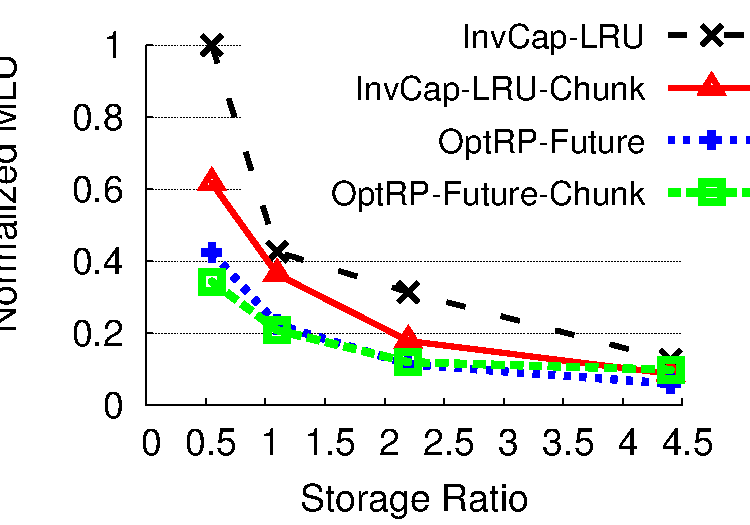
\includegraphics[scale=0.5]{graphSet1/chunkcomp/AbileneVideos.pdf}}
\subfigure[Entertainment trace - ATT] {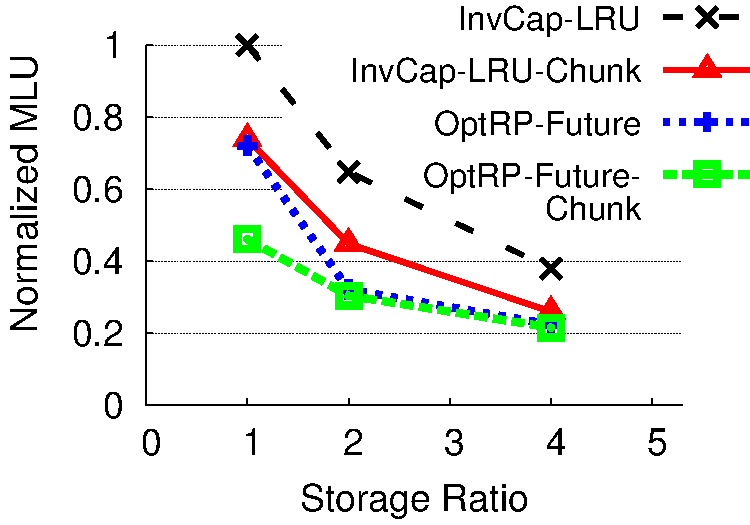
\includegraphics[scale=0.5]{graphSet1/chunkcomp/ATTVideos.pdf}}
\end{center}
\caption{Content chunking improves performance of \invlru\ relative to \optrpfuture\ on both topologies.}
\label{fig:chunking}
\end{figure}


\eat
{
\begin{figure*}[t]
\begin{center}
\subfigure[Entertainment - Abilene] {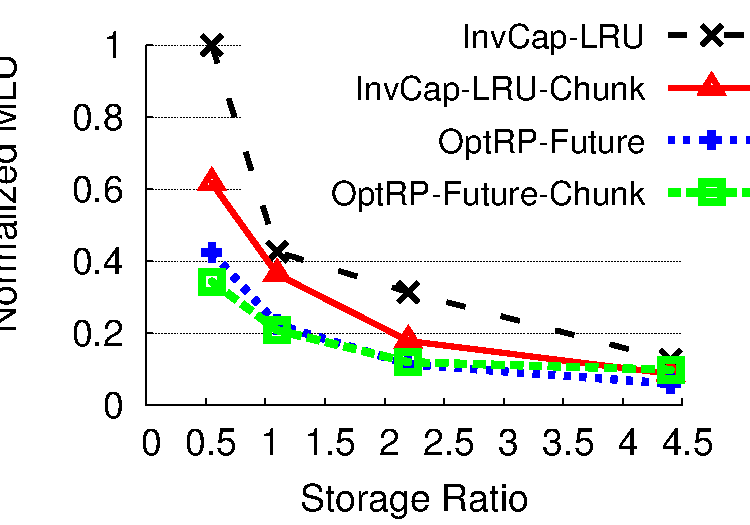
\includegraphics[scale=0.65]{graphSet1/chunkcomp/AbileneVideos.pdf}}
\subfigure[Entertainment - ATT] {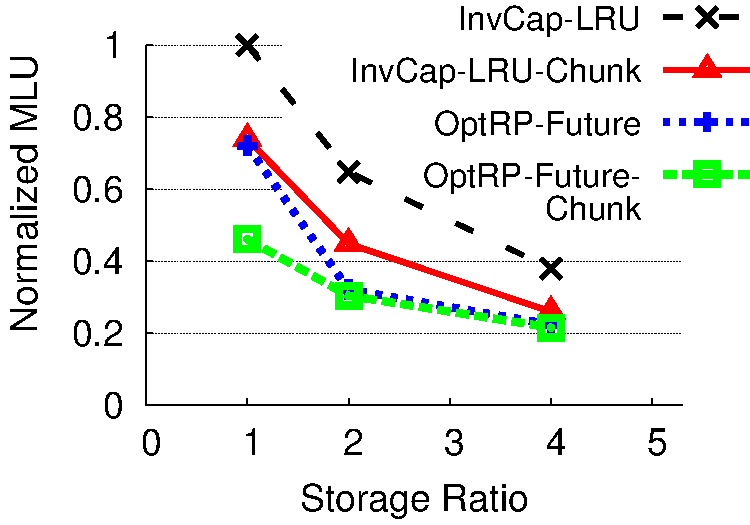
\includegraphics[scale=0.65]{graphSet1/chunkcomp/ATTVideos.pdf}}
\subfigure[Downloads - Abilene] {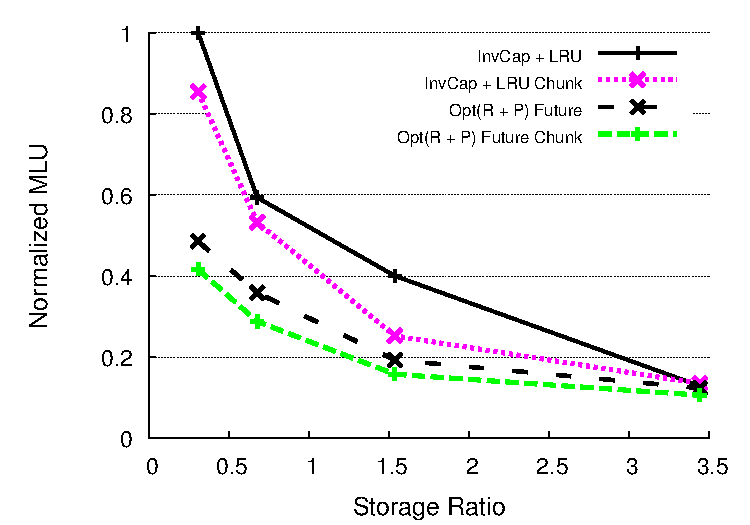
\includegraphics[scale=0.65]{graphSet1/chunkcomp/AbileneDownloads.pdf}}
\subfigure[Downloads - ATT] {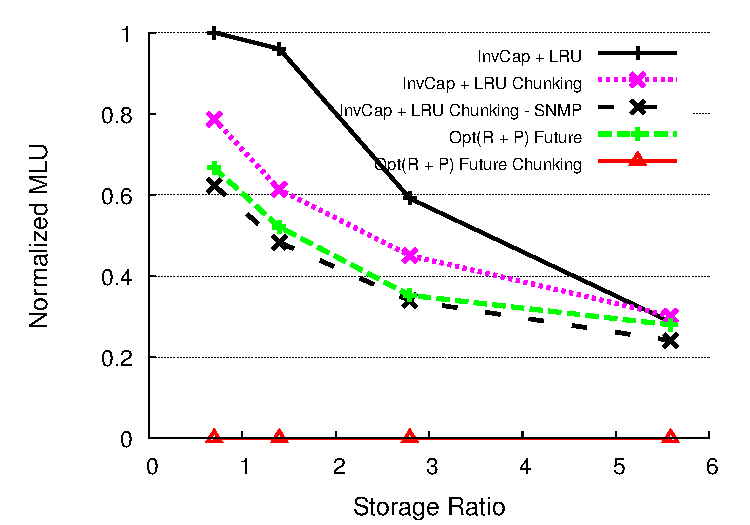
\includegraphics[scale=0.65]{graphSet1/chunking/ATTDownloads.pdf}}
\end{center}
\caption{Content chunking improves performance of \invlru\ relative to \optrpfuture\ on both topologies, strengthening our conclusion that a demand-oblivious content placement and routing suffices for an \ncp.}
\label{fig:chunking}
\end{figure*}

%\begin{figure*}[t]
%\begin{center}
%\subfigure[Entertainment - Abilene] {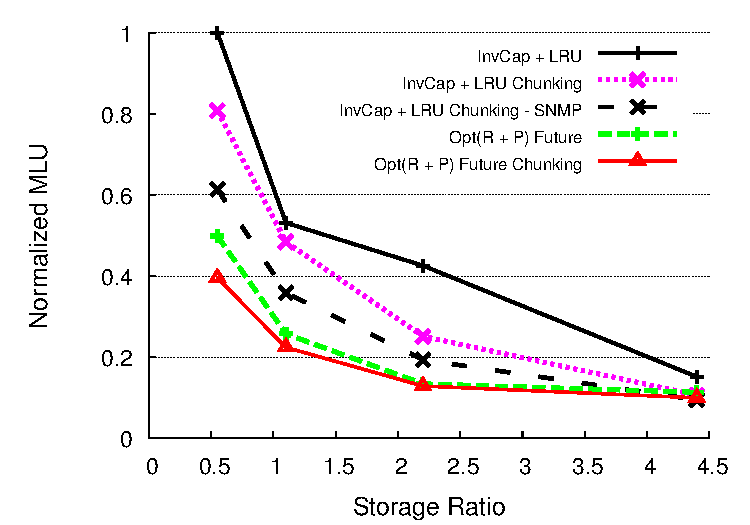
\includegraphics[scale=0.65]{graphSet1/chunking/AbileneVideos.pdf}}
%\subfigure[Entertainment - ATT] {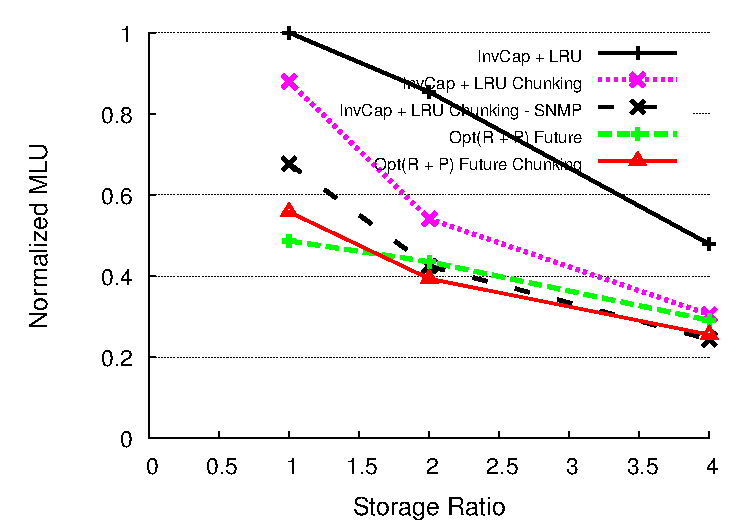
\includegraphics[scale=0.65]{graphSet1/chunking/ATTVideos.pdf}}
%\subfigure[Downloads - Abilene] {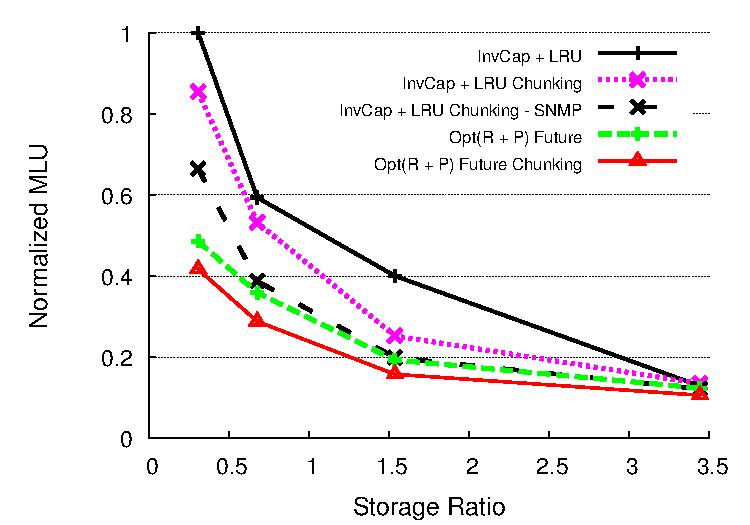
\includegraphics[scale=0.65]{graphSet1/chunking/AbileneDownloads.pdf}}
%\subfigure[Downloads - ATT] {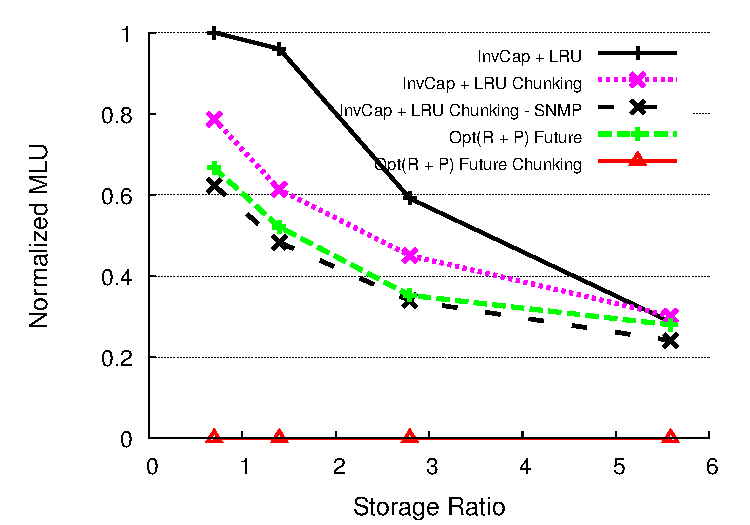
\includegraphics[scale=0.65]{graphSet1/chunking/ATTDownloads.pdf}}
%\end{center}
%\caption{Content chunking improves performance of \invlru\ compared to \optrpfuture\ on both topologies, strengthening our conclusion that a demand-oblivious content placement and routing suffice for a \ncp.}
%\label{fig:chunking}
%\end{figure*}
}

Content chunking is widely used to improve content delivery efficiency. For example, HTTP supports chunked mode transfer \cite{rfc2616}  and BitTorrent distributes content in small chunks \cite{bittorrentprotocol}. In our context, both demand-aware and demand-oblivious placement benefit from chunking. A demand-oblivious placement improves with chunking because  a cache can store a partially downloaded content if a user aborts the download before completion. Chunking helps demand-aware placement for multiple reasons. First, chunks of a content differ in popularity. Therefore,  placing more popular chunks at more locations is better. Second, chunking enables storing more content at each node, e.g., a large file may not  fit at any PoP due to storage constraints,  but its chunks can be stored across a set of PoPs.  Third, splitting a content across multiple locations spreads the traffic for that content over more links, which reduces network cost. 

Our chunking procedure is described in $\S$\ref{sec:simulations}.  While chunking improves performance of both \invlru\ and \optrpfuture, it significantly improves the performance of \invlru\ relative to \optrpfuture. Figure \ref{fig:chunking} shows the results of our experiments on entertainment trace.  Due to chunking, the maximum difference between the MLU of  \invlru\ and \optrpfuture\ reduces from 2.5$\times$ to 1.4$\times$. At the maximum storage ratio in each case, \invlru\ has less than 20\% higher MLU compared to \optrpfuture\ with chunking. Our experiments on the downloads trace have qualitatively similar conclusions (graphs omitted for brevity). Chunking makes a small difference on our experiments with news trace as  more than 95\% content is of duration less than our chunk size.  Hence, chunking strengthens our conclusion that a demand-oblivious placement and routing achieve close to the best possible network cost for an NCDN.


%\invlru\ has up to 2.5$\times$ the MLU compared to \optrpfuture\ without chunking. With chunking,  \invlru\ has only up to 1.4$\times$ the MLU compared to \optrpfuture. At storage ratio of 4, \invlru\ has less than 20\% higher MLU compared to \optrpfuture\ with chunking. 





%On Abilene topology, the maximum difference between \invlru\ and \optrpfuture\ reduces from 2.8$\times$ to 1.6$\times$  at storage ratios $\leq$ 2.2; on ATT topology, the maximum difference reduces  from  2$\times$ to  1.3$\times$ at storage ratios $\leq$ 2. At storage ratios $\geq$ 4, the difference between them is $< 20\%$ on all traces.






\eat
{
We show the effect of content chunking on \invlru\ and \optrpfuture\ in Figure \ref{fig:chunking} . Content chunking significantly improves the performance of \invlru\ relative to \optrpfuture\ on the entertainment trace and the downloads trace for both topologies. On Abilene topology, the maximum difference between \invlru\ and \optrpfuture\ reduces from 2.8$\times$ to 1.6$\times$  at storage ratios $\leq$ 2.2; on ATT topology, the maximum difference reduces  from  2$\times$ to  1.3$\times$ at storage ratios $\leq$ 2. At storage ratios $\geq$ 4, the difference between them is $< 20\%$ on all traces.
}

Even with content chunking, demand-aware placement and routing,  \optrp, has up to 7$\times$ higher network cost compared to \invlru\ in the experiment with entertainment trace (not shown in graph). This is because the reduction in MLU due to content chunking is far exceeded by  the increase in MLU due to the "miss" traffic on the network.

%%This is because the increase in MLU due to the "miss" traffic on the network for \optrp\  far exceeds the gain in efficiency due to content chunking.





%The experiments so far  suggest that a placement strategy that optimizes placement daily only the previous day's history to place content in the network performs poorly in all experiments because new content added to the network results in a significant ``miss'' traffic on the network resulting in large MLUs. 

\subsubsection{Alternative Demand-aware Schemes}
The experiments so far  suggest that a demand-aware scheme that engineers placement and routing once a day based on the previous day's demand performs poorly compared to a demand-oblivious scheme, \invlru. Therefore, in this section, we evaluate the performance of two alternative demand-aware schemes. First is a hybrid scheme that combines demand-aware  and demand-oblivious schemes, and second is a demand-aware scheme that optimizes placement and routing multiple times a day. We discuss each of them in turn.

%A demand-aware scheme that optimizes placement and routing once a day based on the previous day's demand performs significantly worse than a simple demand-oblivious strategy. Is there an alternative demand-aware scheme that consistently outperforms a demand-oblivious scheme, \invlru?  To answer this, we consider two variants of demand-aware schemes. 

%We find that neither of these schemes outperform \invlru.
 
%We explore two such strategies, 



\begin{figure}[t]
\begin{center}
\subfigure[News trace - Abilene]{
	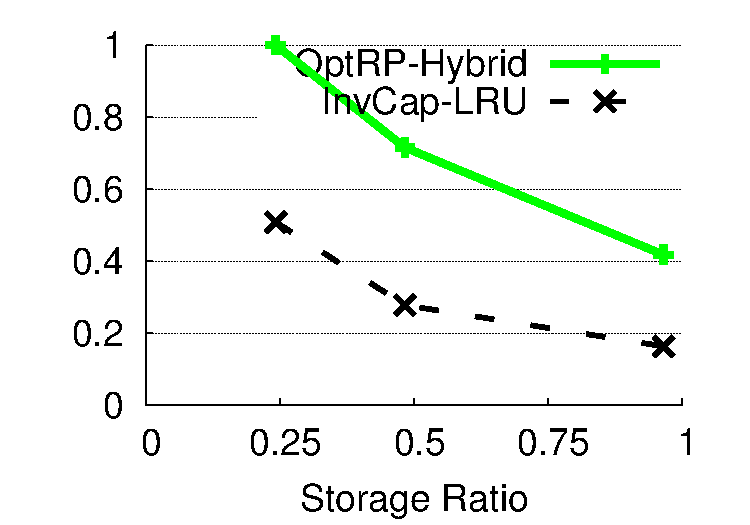
\includegraphics[scale=0.4]{graphSet1/hybrid/AbileneNews.pdf}
}
\subfigure[Entertainment trace - Abilene]{
	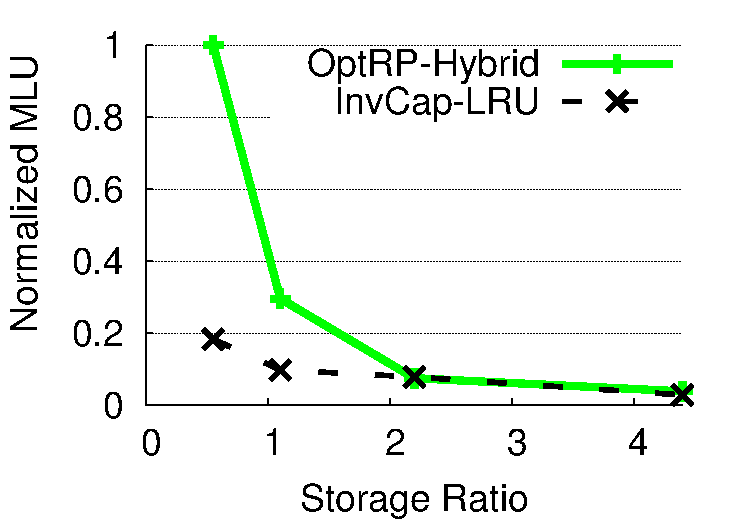
\includegraphics[scale=0.4]{graphSet1/hybrid/AbileneVideos.pdf}
}
\caption{Hybrid placement strategies either perform as well as \invlru\ or worse for both traces.}
\label{fig:hybrid}
\end{center}

\end{figure}


\begin{figure}[t]
\begin{center}
\subfigure[News trace]{
	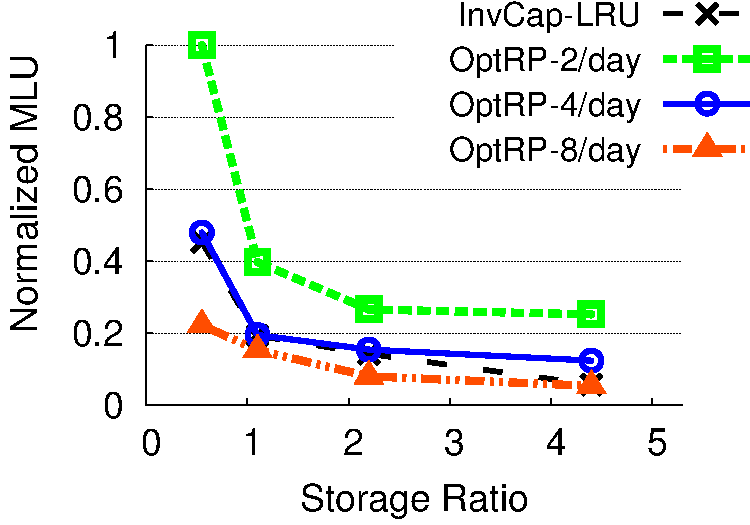
\includegraphics[scale=0.5]{graphSet1/tefrequency/AbileneVideos.pdf}
}
\subfigure[Entertainment trace]{
	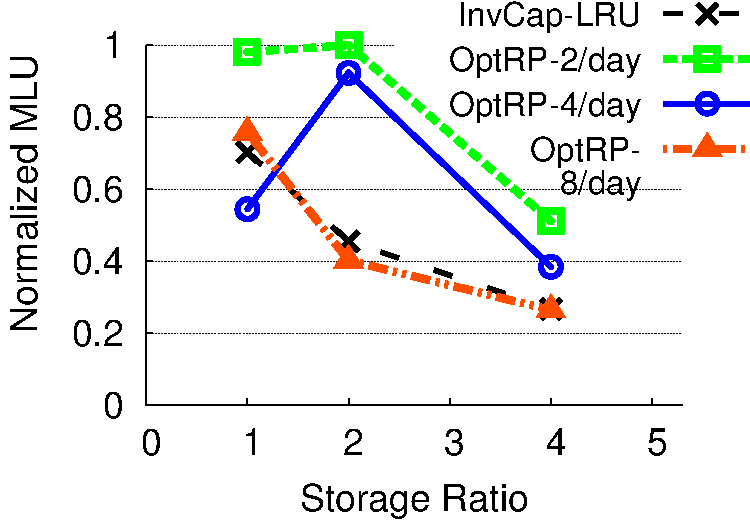
\includegraphics[scale=0.5]{graphSet1/tefrequency/ATTVideos.pdf}
}
\caption{Demand-aware placement and routing can match the performance of \invlru\ if computed eight times per day.}
\label{fig:optrpfrequency}
\end{center}
\end{figure}


\textbf{Hybrid placement:} We evaluate a hybrid placement scheme, which splits the storage at each node into two parts - one for a demand-aware placement based on previous day's content demand and the other for placing the content in a demand-oblivious LRU manner. This hybrid strategy is similar to that used in \cite{Applegate2010}. We present the results for experiments with news trace and entertainment trace on the Abilene topology in Figure \ref{fig:hybrid}. For this experiment, we used 20\% of storage at each node as a LRU cache and the rest of the storage to place content exactly as in \optrp. We find that in both these cases \invlru\ performs either as well or better than the \optrp\ scheme.  We also experimented with assigning a greater fraction of storage to demand-oblivious placement (omitted for brevity), but the above conclusions remain unchanged in those experiments.


%The experiments so far  suggest that a placement strategy that uses only the previous day's history to place content in the network performs poorly in all experiments because new content added to the network results in a significant ``miss'' traffic on the network resulting in large MLUs. Therefore, in this section, we evaluate the performance of hybrid placement strategies, which split their storage at each node into two parts - one for a demand-aware placement based on previous day's content demand and the other for placing the content in a demand-oblivious LRU manner. This hybrid strategy is similar to that used in \cite{Applegate2010}.


This experiment shows that simple strategies that combine demand-oblivious placement and demand-aware placement do not perform better than a demand-oblivious content placement scheme. Of course, a carefully designed hybrid placement scheme by definition should perform at least as well as the demand-oblivious and demand-aware schemes, both of which are extreme cases of a hybrid strategy. However, we were unable to design simple hybrid strategies that consistently outperformed fully demand-oblivious placement and routing.





\textbf{\optrp\ multiple times per day:} Next, we analyze the performance of demand-aware schemes that engineer placement and routing multiple times each day at equal intervals - twice per day, four times per day, and eight times per day. In all cases, we use the content demand in the past 24 hours to engineer placement and routing. In Figure \ref{fig:optrpfrequency}, we compare the performance \optrp\ for different frequencies against \invlru\ scheme. As \optrp\ engineers more frequently, its performance improves. This is because it updates placement more quickly based on the demand for new content and a change in demand for older content. However, \optrp\ needs to engineer eight times per day to match the performance of a demand-oblivious placement. In other cases, \invlru\ performs better.
 
Considering the effort of executing a demand-aware placement - measuring content demand at all PoPs, solving a time-consuming optimization problem, moving content to new locations - and the frequency at which it needs to be done - eight times a day, it seems that demand-aware placement is difficult to implement. In comparison, a demand-oblivious placement requires much less effort on part of the NCDN and on provisioning more storage (storage ratio of 4 in most cases) achieves network cost close to \optrpfuture\ scheme.


%Executing a demand-aware placement requires additional effort - measuring content demand, solving a time-consuming optimization problem, moving content to new locations - over a demand-oblivious placement. Moreover, demand-aware scheme needs to be done eight times a day for it to do better than a demand-oblivious placement. 


%and the frequency at which it needs to be done - eight times a day, demand-aware placement is difficult to implement. In comparison, a demand-oblivious placement requires much less effort on part of the NCDN and on provisioning more storage (storage ratio of 4 in most cases) achieves network cost close to the best possible.




%whether the update interval is 6 hours, 12 hours, or 24 hours makes only a small difference to \optrp's performance, while an update interval of 72 hours results in a significantly higher network cost.  Reducing the update interval from 24 hours to 6 or 12 hours does not lower the MLU  significantly because the new content published between two placement and routing updates still results in a high MLU for \optrp. On increasing the update interval from 24 hours to 72 hours, \optrp\ becomes much less responsive to new content and hence its MLU is even higher.

%If a demand-aware placement is updated once-a-day, 


%We first investigate how the frequency at which demand-aware placement and routing is updated affect its performance.  We vary the interval at which \optrp\ updates its placement and routing to 6 hours, 12 hours, 24 hours, and 72 hours. In earlier experiments, this interval was set to 24 hours. We decide placement and routing in all cases based on the content demand in the past 24 hours. As Figure \ref{fig:optrpfrequency} shows, whether the update interval is 6 hours, 12 hours, or 24 hours makes only a small difference to \optrp's performance, while an update interval of 72 hours results in a significantly higher network cost.  Reducing the update interval from 24 hours to 6 or 12 hours does not lower the MLU  significantly because the new content published between two placement and routing updates still results in a high MLU for \optrp. On increasing the update interval from 24 hours to 72 hours, \optrp\ becomes much less responsive to new content and hence its MLU is even higher.





%achieving a demand-aware placement an uphill task. A demand-oblivious placement requires much less effort on part of the NCDN and at a storage ratio of 4 in most cases can match the performance of a demand-aware placement with perfect knowledge. 

% At moderate storage ratios, a demand-oblivious strategy already performs close to a demand-aware strategy which has perfect knowledge of next day's demand.


%Given that a demand-oblivious scheme can already match the performance of demand-aware scheme with perfect knowledge of next day's demand at moderate storage ratios ($\approx$ 4), the case for a demand-aware placement is already weakened.

\eat
{
\label{sec:hybrid}
\subsection{Hybrid Placement} The experiments so far  suggest that a placement strategy that uses only the previous day's history to place content in the network performs poorly in all experiments because new content added to the network results in a significant ``miss'' traffic on the network resulting in large MLUs. Therefore, in this section, we evaluate the performance of hybrid placement strategies, which split their storage at each node into two parts - one for a demand-aware placement based on previous day's content demand and the other for placing the content in a demand-oblivious LRU manner. This hybrid strategy is similar to that used in \cite{Applegate2010}.

We present the results for experiments with the news trace and entertainment trace on the Abilene topology in Figure \ref{fig:hybrid}. For this experiment, we used 20\% of storage at each node as a LRU cache and the rest of the storage to place content exactly as in \optrp. We find that in both these cases \invlru\ performs either as well or better than the \optrp\ scheme. 
We also experimented with assigning a greater fraction of storage to demand-oblivious placement (omitted for brevity), but the above conclusions remain unchanged in those experiments. 

This experiment shows that simple strategies that combine demand-oblivious placement and demand-aware placement do not perform better than a demand-oblivious content placement scheme. Of course, a carefully designed hybrid placement scheme by definition should perform at least as well as the demand-oblivious and demand-aware schemes, both of which are extreme cases of a hybrid strategy. However, we were unable to design simple hybrid strategies that consistently outperformed fully demand-oblivious placement and routing.

}







\subsubsection{Impact of Experimental Parameters}
\label{sec:parameters}

We perform an extensive set of experiments to understand the effect of some of the key parameters such as storage distribution across nodes, frequency of routing updates, and number of exit nodes that connect to the origin. Overall, we find that our key conclusions are robust to variations in the values of these parameters.

%These parameters include storage distribution across nodes, content placement and/or routing update frequency, and number of exit nodes connected to origin.

\eat
{
%%%%% START TO EAT
\textbf{Demand-aware placement and routing (\optrp) parameters:}  We first investigate how the frequency at which demand-aware placement and routing is updated affect its performance.  We vary the interval at which \optrp\ updates its placement and routing to 6 hours, 12 hours, 24 hours, and 72 hours. In earlier experiments, this interval was set to 24 hours. We decide placement and routing in all cases based on the content demand in the past 24 hours. As Figure \ref{fig:optrpfrequency} shows, whether the update interval is 6 hours, 12 hours, or 24 hours makes only a small difference to \optrp's performance, while an update interval of 72 hours results in a significantly higher network cost.  Reducing the update interval from 24 hours to 6 or 12 hours does not lower the MLU  significantly because the new content published between two placement and routing updates still results in a high MLU for \optrp. On increasing the update interval from 24 hours to 72 hours, \optrp\ becomes much less responsive to new content and hence its MLU is even higher. 



%\textbf{HIstory of TE:} We compared the performance of \optrp\ by varying amount of history based on which \optrp\ optimizes content placement and routing. \optrp\ engineers traffic once every 24 hours, but uses content popularity in the past 6 hours, 12 hours, 24 hours, and 72 hours to optimize content placement. 

%the engineering frequency to 6 hours, 12 hours, 24 hours, and 72 hours. In each case, we use the content demand in the past 24 hours to decide demand-aware placement. 

\textbf{Frequency of TE and History of Content Popularity Used by \optrp:} In our experiments until now, \optrp\ used the content popularity on the previous day to calculate demand-aware placement and routing for the next day.  We evaluate \optrp's performance by varying two parameters: (1) how frequently \optrp\ updates placement and routing  (2) how many days of history of content popularity is used to calculate placement and routing.   We experiment with two scenarios for the first parameter - (1) TE is done each day, (2)  TE is done every 3 days - and two scenarios for the second parameter - (1) TE is done using one-day history of content popularity, (2) TE is done using three days history of content popularity.

Our results are shown in Figure \ref{fig:history}. There are two main observations which are consistent across all graphs (1) doing TE every three days performs worse than doing TE each day (2) whether a one-day history  or a three-day history of content popularity is used makes little difference.  These findings imply that varying the above parameters is unlikely to improve the  poor performance of demand-aware placement and routing.


\begin{figure*}[t]
\begin{center}
\subfigure[News videos trace - Abilene] {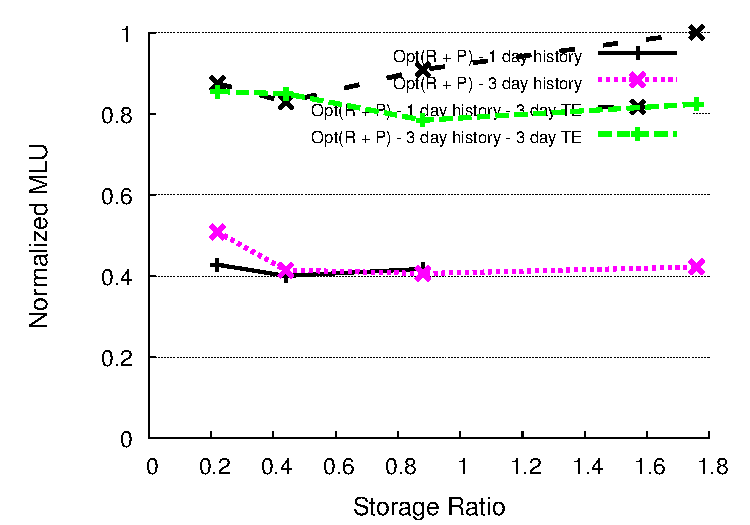
\includegraphics[scale=0.65]{graphSet1/history/AbileneNews.pdf}}
\subfigure[News videos trace - ATT] {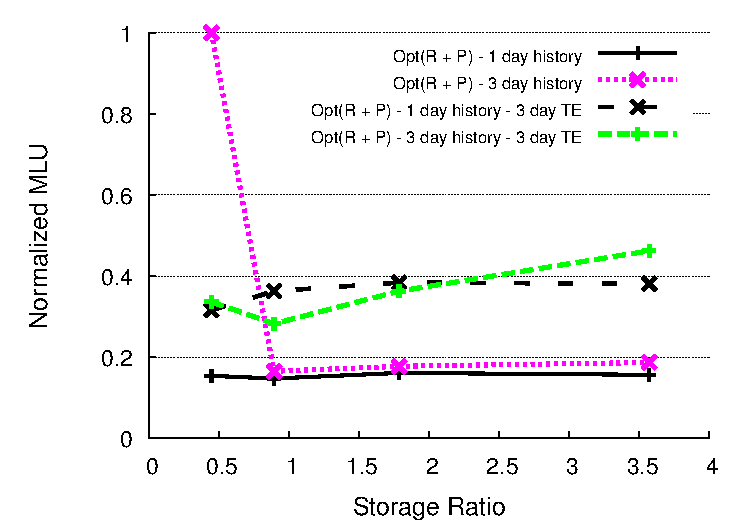
\includegraphics[scale=0.65]{graphSet1/history/ATTNews.pdf}}
\subfigure[Downloads trace - Abilene] {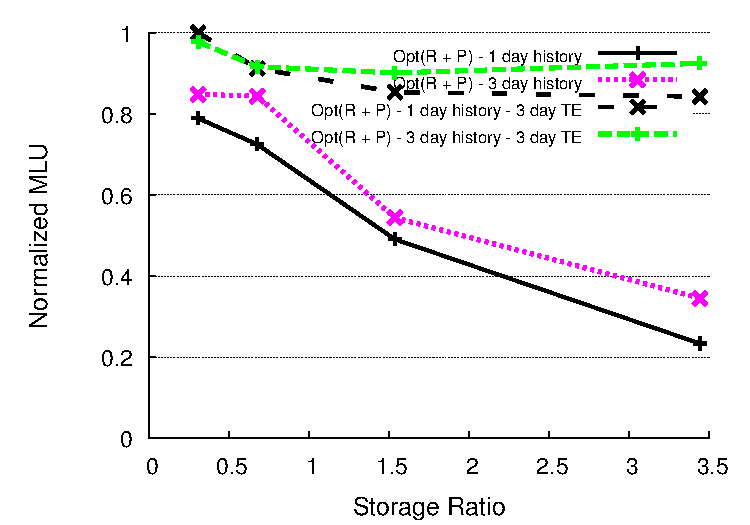
\includegraphics[scale=0.65]{graphSet1/history/AbileneDownloads.pdf}}
\subfigure[Downloads trace - ATT] {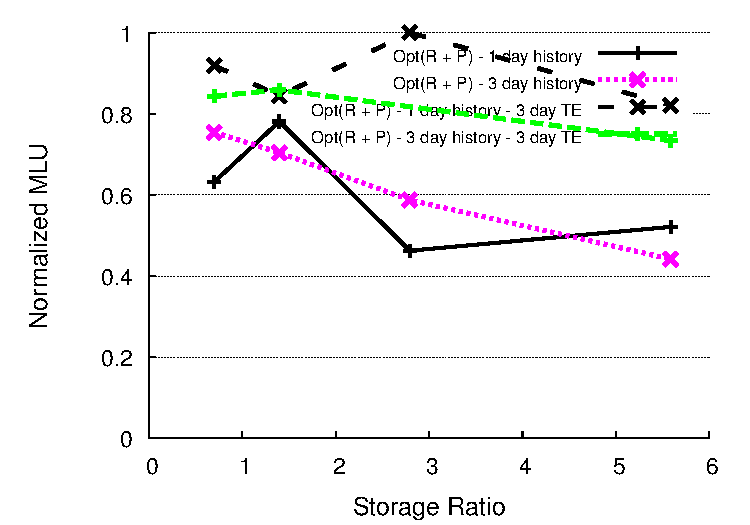
\includegraphics[scale=0.65]{graphSet1/history/ATTDownloads.pdf}}
\end{center}
\caption{Using a 3 day history of content popularity does not improve \optrp's performance over using a one day history of content popularity. Engineering placement and routing every 3 days performs worse than engineering traffic every day.}
\label{fig:history}
\end{figure*}

%%%%% END OF EAT
}

%We have observed that \optlru\ makes little improvement to network cost over \invlru.  Can we improve \optlru's network cost if we optimize routing at a different frequency ? To answer this question, we experimented with three different frequencies of TE - once every 3 hours (default frequency), once every 6 hours, and once every 24 hours. In each case, the optimal routing is computed based on TM measured since the last time TE was done.  In Figure \ref{fig:optrfrequency}, the network cost of \optlru\ for difference frequencies of TE are shown in Figure \ref{fig:optrfrequency}. The legend in this figure shows the frequency of TE, e.g., ``OptR+LRU 3hr'' means TE frequency is once every 3 hours. Our conclusion is that the performance of \optlru\ remains the nearly same irrespective of the TE frequency. 
 
\textbf{Demand-aware routing (\optlru) parameters:} While \optlru\ has nearly the same network cost as \invlru, but does \optlru\ perform better if we change the interval at which routing is updated, or we optimize routing based on a traffic matrix other than the one measured over the past three hours.  We perform two sets of experiments to answer this question. The first experiment varies the routing update interval from 3 hours (default value) to 6 hours and to  1 day. In each case, we compute routing based on TM measured since the last routing update.  We find that the network cost of \optlru\ remains almost unchanged irrespective of the routing update interval (graphs omitted for brevity). The  second experiment  optimizes routing based on the TM measured on the previous day instead of TM measured since the last routing update, e.g., if routing is being updated at 9am for the period of 9am-12pm, then we use TM measured from 9am-12pm on the previous day.  We set the routing update interval to 3 hours and then to 6 hours. We find that the network cost in in both these cases is nearly identical to \optlru's network cost with our default parameters (graphs omitted for brevity). This experiment suggests that \optlru\ is unlikely to improve even if we optimize routing based on other previously measured TMs.  In summary, these experiments reinforce the finding that \invlru\ is as effective as \optlru.



\eat
{

In Figure \ref{fig:optrprevdaytm}, we show the network of ``OptR+LRU 3hr prevday'' and ``OptR+LRU 6hr prevday'', which optimize routing every three hours and every six hours respectively based on TM measured the previous day. For comparison, we also plot ``OptR+LRU 1d'' scheme from Figure \ref{fig:optrfrequency}. ``OptR+LRU 3hr prevday'' and ``OptR+LRU 6hr prevday'' have nearly the same network cost as ``OptR+LRU 1d'' scheme which shows that using TM measured on previous day does not affect our conclusions. 



%In Figure \ref{fig:optrfrequency}, the network cost of \optlru\ for difference frequencies of TE are shown in Figure \ref{fig:optrfrequency}. The legend in this figure shows the frequency of TE, e.g., ``OptR+LRU 3hr'' means TE frequency is once every 3 hours. Our conclusion is that the performance of \optlru\ remains the nearly same irrespective of the TE frequency.

First, we experimented with three different frequencies of TE - once every 3 hours (default frequency), once every 6 hours, and once every 24 hours. In each case, the optimal routing is computed based on TM measured since the last time TE was done.  In Figure \ref{fig:optrfrequency}, the network cost of \optlru\ for difference frequencies of TE are shown in Figure \ref{fig:optrfrequency}. The legend in this figure shows the frequency of TE, e.g., ``OptR+LRU 3hr'' means TE frequency is once every 3 hours. Our conclusion is that the performance of \optlru\ remains the nearly same irrespective of the TE frequency.

Next, we optimize routing using the TM measured on the previous day instead of TM measured since the last time routing was updated. For example, if routing is being done for 9am-12pm today, then we use TM measured from 9am-12pm on the previous day.  In Figure \ref{fig:optrprevdaytm}, we show the network of ``OptR+LRU 3hr prevday'' and ``OptR+LRU 6hr prevday'', which optimize routing every three hours and every six hours respectively based on TM measured the previous day. For comparison, we also plot ``OptR+LRU 1d'' scheme from Figure \ref{fig:optrfrequency}. ``OptR+LRU 3hr prevday'' and ``OptR+LRU 6hr prevday'' have nearly the same network cost as ``OptR+LRU 1d'' scheme which shows that using TM measured on previous day does not affect our conclusions. 



%In the second experiment, we optimize routing based on TM measured on the previous day in the interval for which routing is being computed. 



%Next, we compared the network cost when we optimize routing using traffic matrix measured on previous day instead of traffic matrix measured on the next day. 

%We performed two sets of experiments. In the first experiment, we varied the frequency of TE - once every 3 hours, once every 6 hours, once every 24 hours. 

%\optlru\ calculates optimizes routing periodically (once every 3 hours) based on previously measured TM (average TM over the past 3 hours). 



\begin{figure*}[t]
\begin{center}
\subfigure[News trace - Abilene] {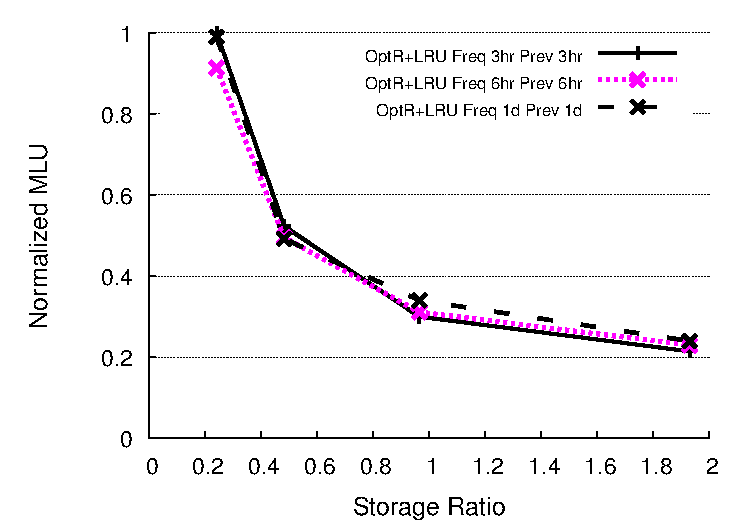
\includegraphics[scale=0.65]{graphSet1/optrteinterval/AbileneNews.pdf}}
\subfigure[News trace - ATT] {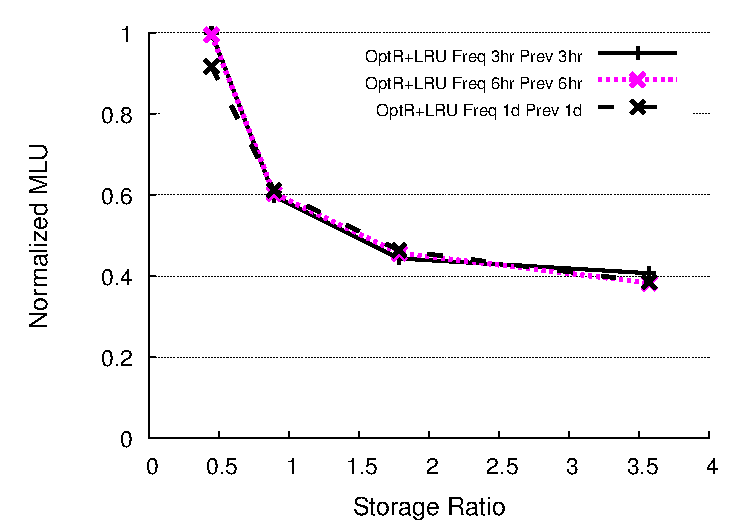
\includegraphics[scale=0.65]{graphSet1/optrteinterval/ATTNews.pdf}}
\subfigure[Entertainment trace - Abilene] {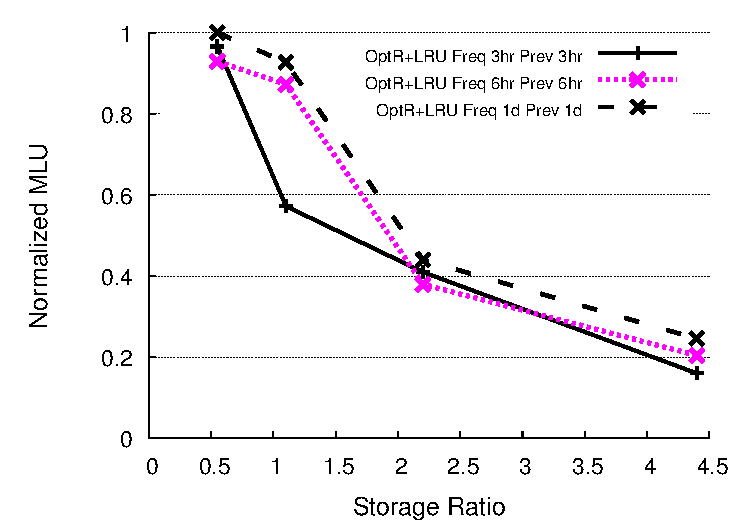
\includegraphics[scale=0.65]{graphSet1/optrteinterval/AbileneVideos.pdf}}
\subfigure[Entertainment trace - ATT] {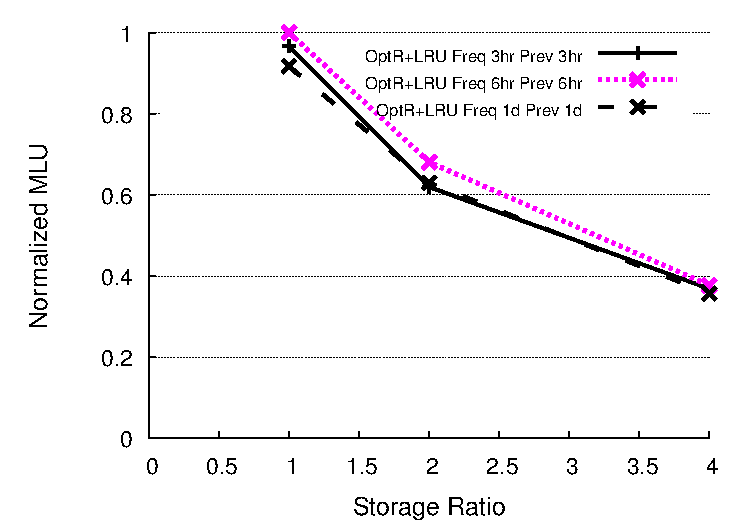
\includegraphics[scale=0.65]{graphSet1/optrteinterval/ATTVideos.pdf}}
\subfigure[Downloads trace - Abilene] {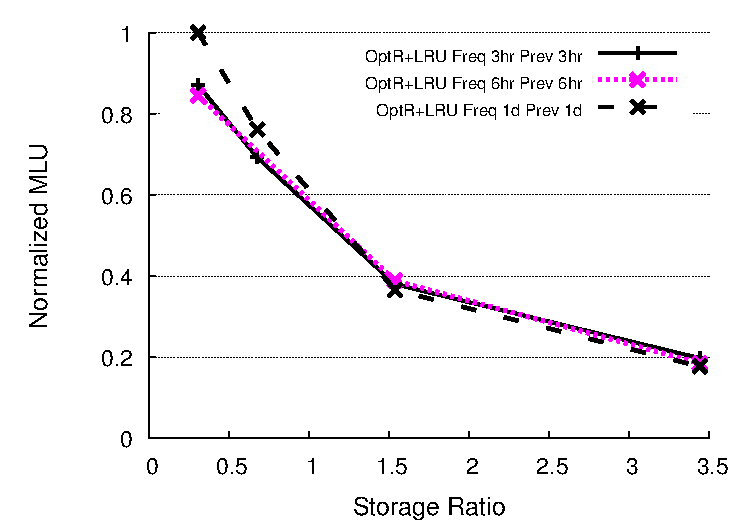
\includegraphics[scale=0.65]{graphSet1/optrteinterval/AbileneDownloads.pdf}}
\subfigure[Downloads trace - ATT] {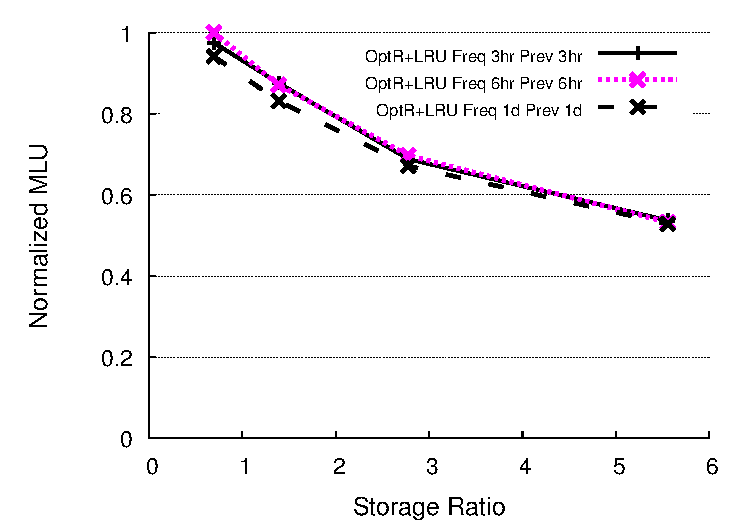
\includegraphics[scale=0.65]{graphSet1/optrteinterval/ATTDownloads.pdf}}
\end{center}
\caption{Varying the frequency of TE for \optlru.}
\label{fig:optrfrequency}
\end{figure*}


\begin{figure*}[t]
\begin{center}
\subfigure[News videos trace - Abilene] {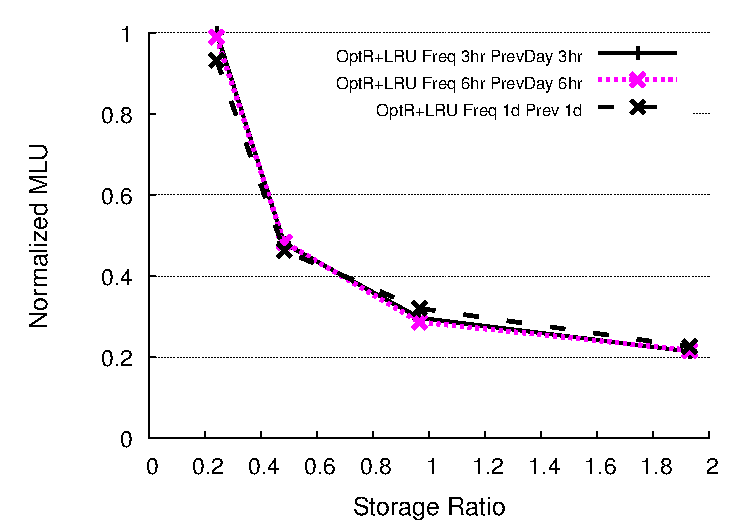
\includegraphics[scale=0.65]{graphSet1/optrtehistory/AbileneNews.pdf}}
\subfigure[News videos trace - ATT] {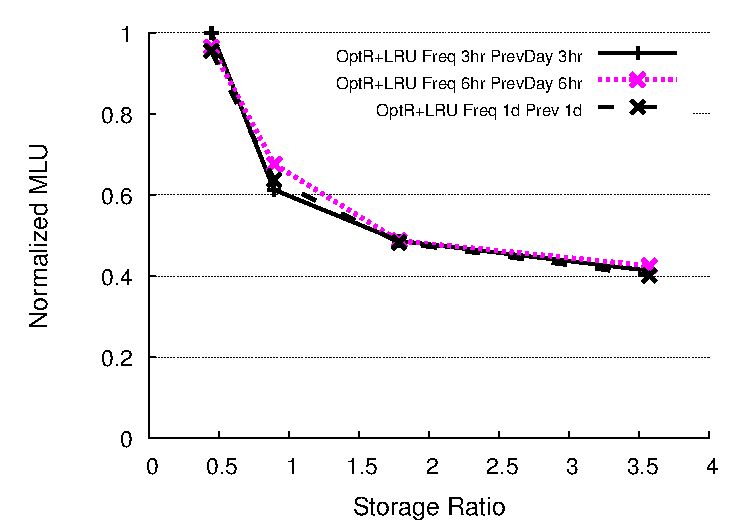
\includegraphics[scale=0.65]{graphSet1/optrtehistory/ATTNews.pdf}}
\subfigure[Entertainment trace - Abilene] {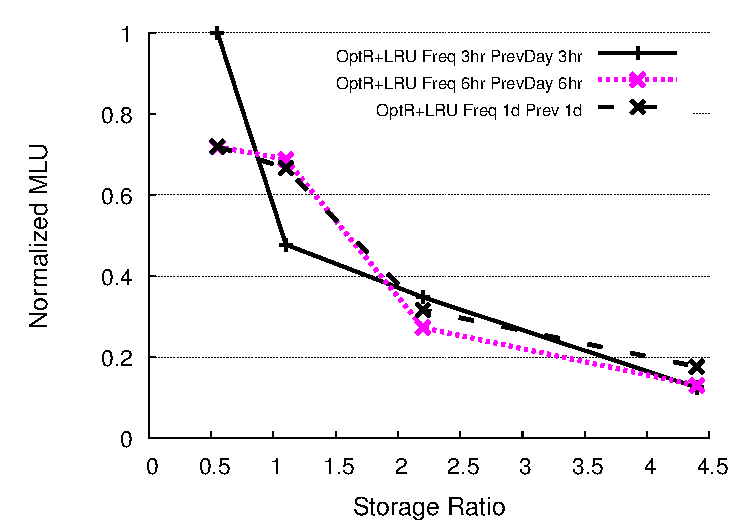
\includegraphics[scale=0.65]{graphSet1/optrtehistory/AbileneVideos.pdf}}
\subfigure[Entertainment trace - ATT] {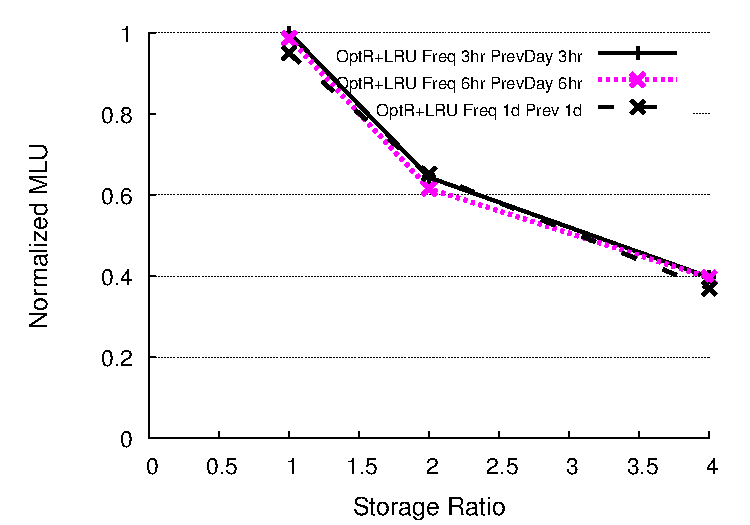
\includegraphics[scale=0.65]{graphSet1/optrtehistory/ATTVideos.pdf}}
\subfigure[Downloads trace - Abilene] {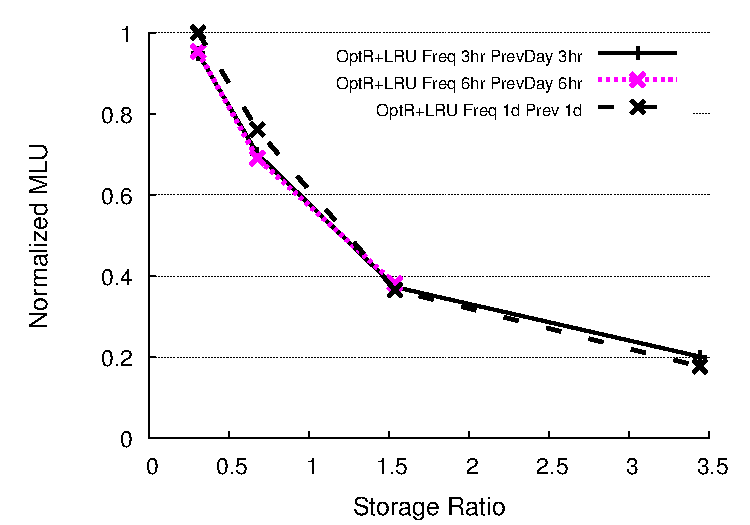
\includegraphics[scale=0.65]{graphSet1/optrtehistory/AbileneDownloads.pdf}}
\subfigure[Downloads trace - ATT] {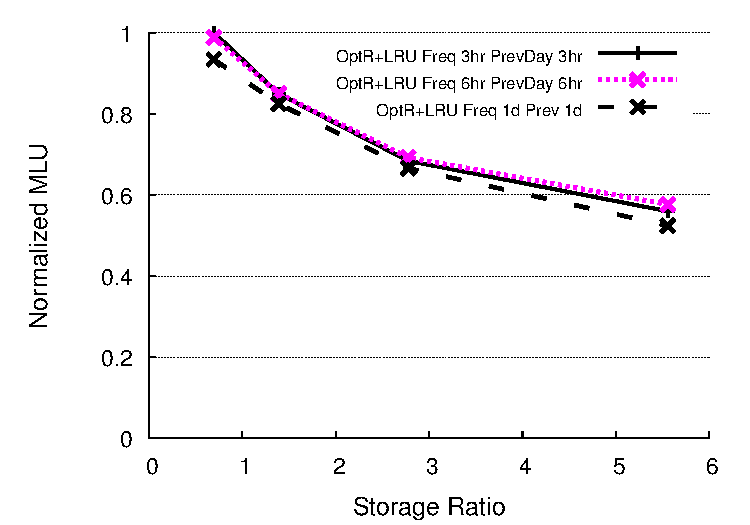
\includegraphics[scale=0.65]{graphSet1/optrtehistory/ATTDownloads.pdf}}
\end{center}
\caption{Doing TE using previous day's TMs.}
\label{fig:optrprevdaytm}
\end{figure*}

}

\textbf{Heterogenous storage:}  In this experiment, the storage at each PoP is set proportional to the fraction of requests at the PoP in each trace. We repeat our experiments keeping storage ratios the same as before. %Our results are shown in Figure \ref{fig:hetpop}. 
We draw out two main observations from our results (graphs omitted for brevity). First, \optrp\ continues to perform poorly compared to \invlru. This is expected as heterogenous storage makes little difference to the ``miss'' traffic generated because of newly published content. Second, for the same storage ratio, network cost increases for both  \invlru\ and  \optrpfuture\ but the increase is more for \invlru\ compared to \optrpfuture. We observe that \invlru's network cost increases up to 30\% or more in four out of six experiments. But \optrpfuture's network cost increases up to 20\% or less (except for entertainment trace on ATT topology).  The increase in \invlru's network cost is likely because the PoPs that have the smallest fraction of all requests are assigned extremely small storage, which increases cache miss rate at these PoPs. Therefore, homogenous storage at PoPs is preferable as it achieves a lower network cost than this heterogenous storage distribution.

%As a result, the difference between \invlru\ and \optrpfuture\ increases.

We evaluated \invlru's performance with two more heterogenous storage distributions: (1) storage proportional to capacity of outgoing links at PoP (2) storage proportional to the number of outgoing links at PoP. Compared to a homogenous storage, the network cost of \invlru\ is up to 180\% more when storage is set proportional to capacity and is up to 60\% more when storage is set proportional to number of degree of the PoP. A heterogenous storage distribution which improves \invlru's network cost over a homogenous storage distribution  is unclear to us at this moment.

%disproportionately reduces the cache size for a few nodes

%This experiment also implies that a homogenous storage distribution achieves a lower network cost for \ancp\ compared to the current heterogenous storage distribution. 




\eat
{

\begin{figure*}[t]
\begin{center}
\subfigure[News trace - Abilene] {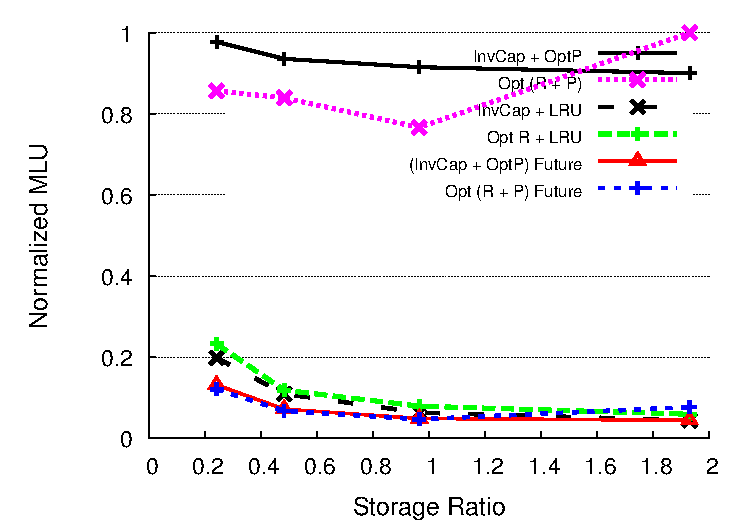
\includegraphics[scale=0.65]{graphSet1/hetpop/AbileneNews.pdf}}
\subfigure[News trace - ATT] {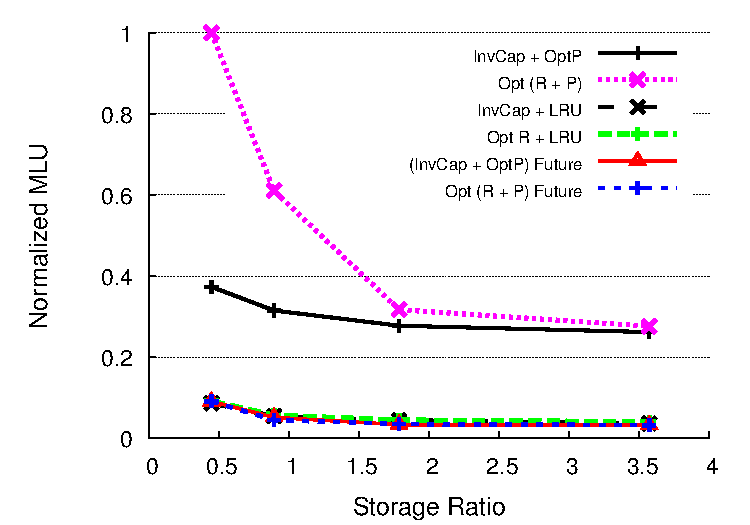
\includegraphics[scale=0.65]{graphSet1/hetpop/ATTNews.pdf}}
\subfigure[Entertainment trace - Abilene] {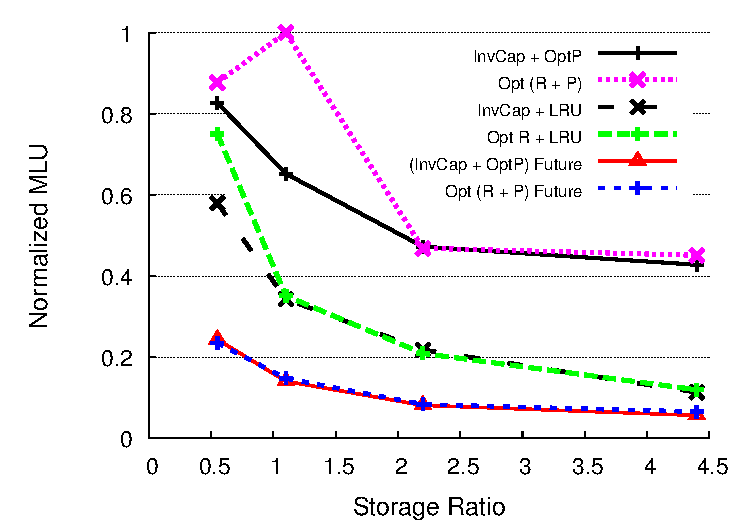
\includegraphics[scale=0.65]{graphSet1/hetpop/AbileneVideos.pdf}}
\subfigure[Entertainment trace - ATT] {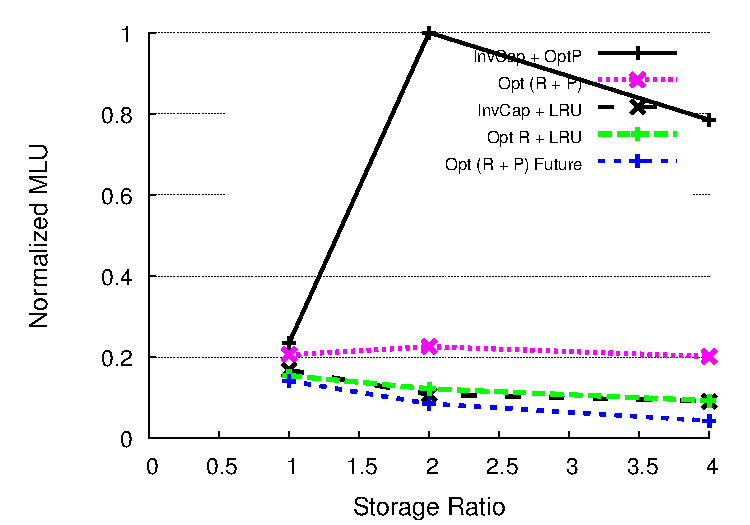
\includegraphics[scale=0.65]{graphSet1/hetpop/ATTVideos.pdf}}
\subfigure[Downloads trace - Abilene] {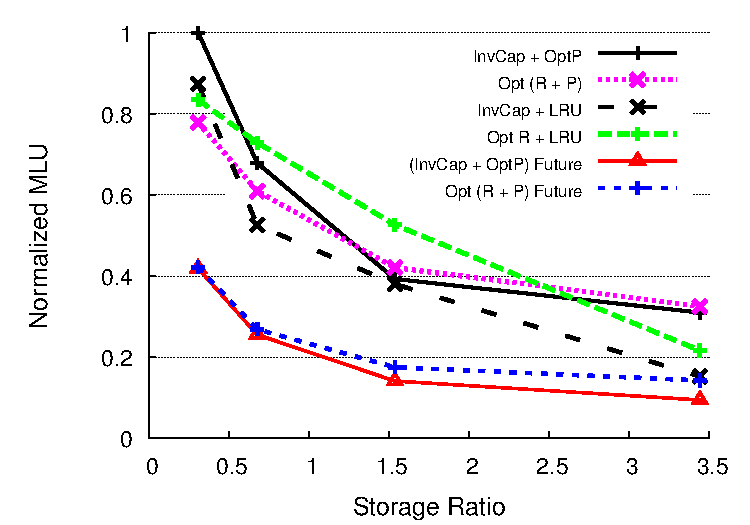
\includegraphics[scale=0.65]{graphSet1/hetpop/AbileneDownloads.pdf}}
\subfigure[Downloads trace - ATT] {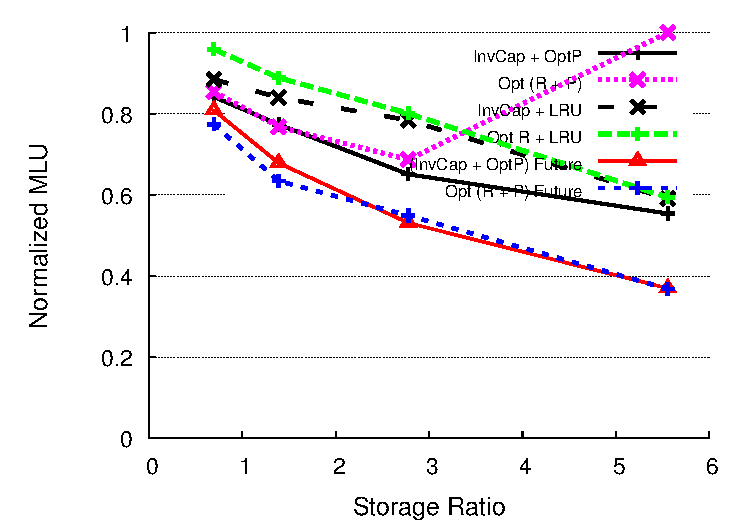
\includegraphics[scale=0.65]{graphSet1/hetpop/ATTDownloads.pdf}}
\end{center}
\caption{Heterogenous storage does not improve the performance of \optrp. \invlru\ performs worse with heterogenous storage compared to homogenous storage, which increases the difference between   \optrpfuture\ and \invlru.}
\label{fig:hetpop}
\end{figure*}
}


%\begin{figure}[t]
%\begin{center}
%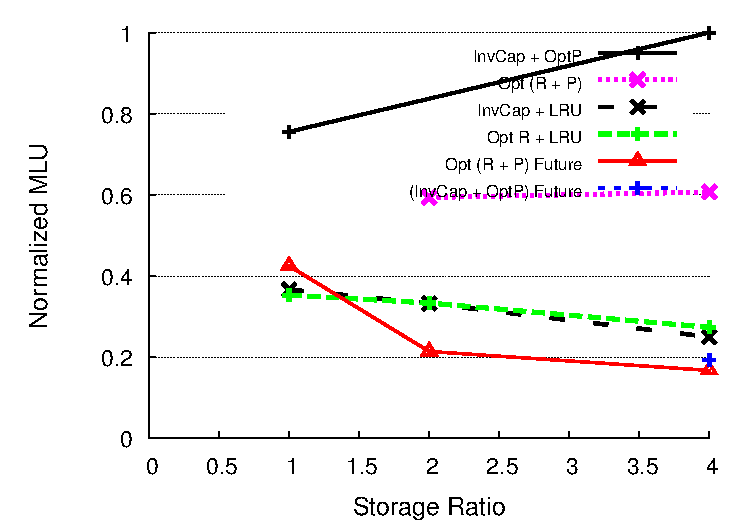
\includegraphics[scale=0.65]{graphSet1/hetero/ATTVideos.pdf}
%\end{center}
%\caption{Heterogenous storage distribution. Entertainment videos trace on ATT topology.}
%\label{fig:hetero}
%\end{figure}



\textbf{Number of exit nodes to origin:}  Until now we have assumed that the origin can be reached from three exit locations in the network.  Next, we perform our experiments with one exit location and five exit locations. Our main findings from the prior sections, namely--\invlru\ performs significantly better than \optrp; \optrpfuture\ performs better than  \invlru; and optimizing routing adds little value;--remain unchanged as we vary the number of exit nodes. Thus, our findings are not sensitive to the number of exit nodes connected to the origin.

%Until now we have assumed origin server can be reached from three exit locations in the network.  Next, we performed our experiments with one exit location and five exit locations. While we find that qualitatively our findings remain unchanged 

%Five origin nodes: Figure \ref{fig:fiveorigins} and Figure \ref{fig:singleorigin}.

\eat{

\begin{figure*}[t]
\begin{center}
\subfigure[News trace - Abilene] {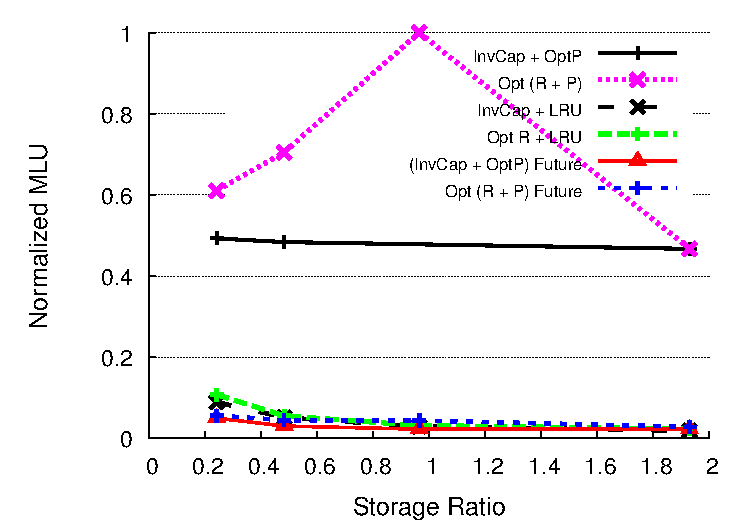
\includegraphics[scale=0.65]{graphSet1/singleoriginnew/AbileneNews.pdf}}
\subfigure[News trace - ATT] {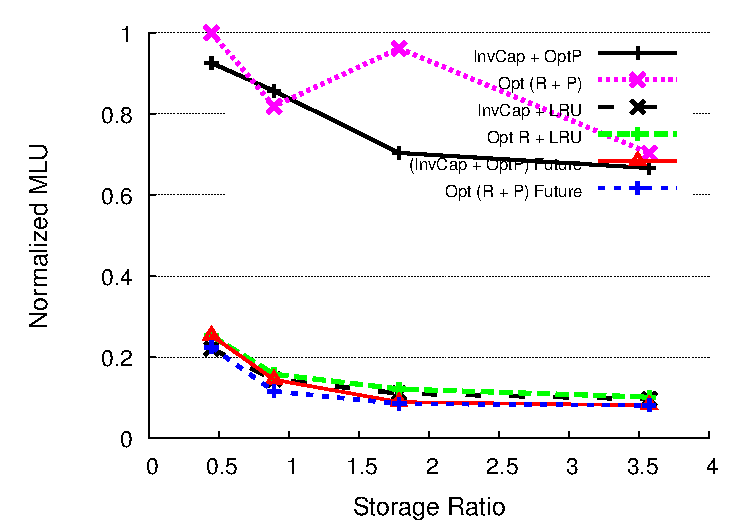
\includegraphics[scale=0.65]{graphSet1/singleoriginnew/ATTNews.pdf}}
\subfigure[Entertainment trace - Abilene] {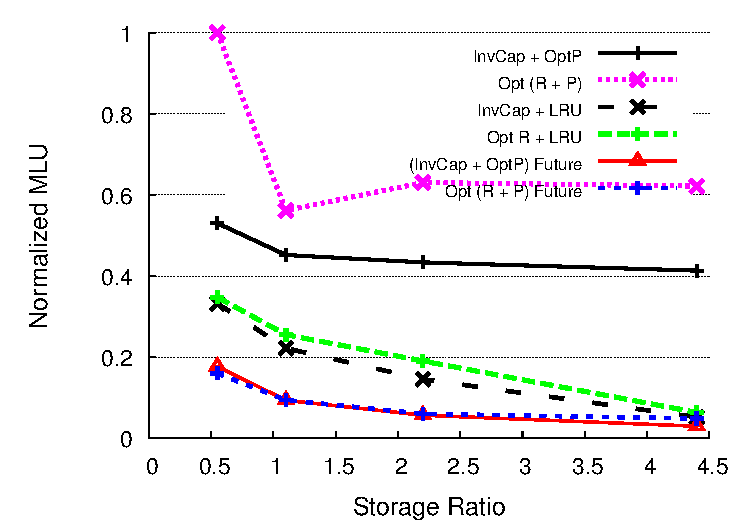
\includegraphics[scale=0.65]{graphSet1/singleoriginnew/AbileneVideos.pdf}}
\subfigure[Entertainment trace - ATT] {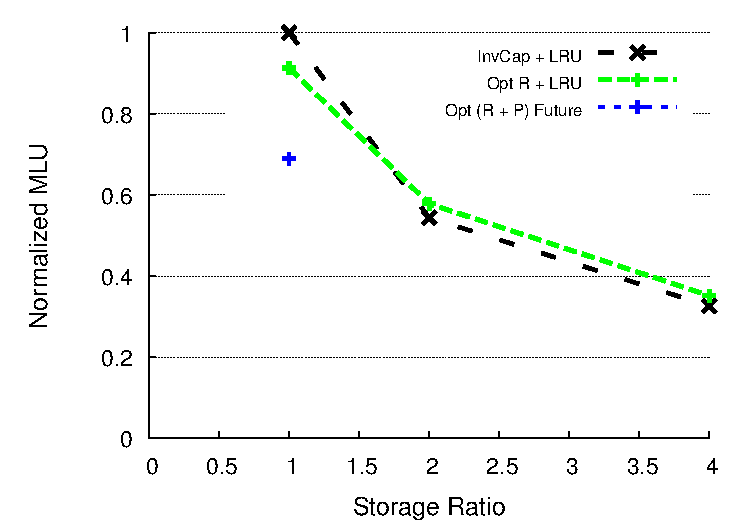
\includegraphics[scale=0.65]{graphSet1/singleoriginnew/ATTVideos.pdf}}
\subfigure[Downloads trace - Abilene] {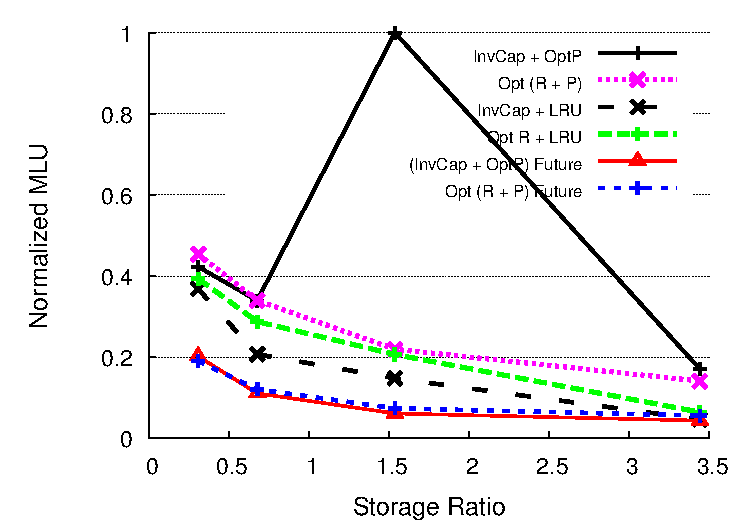
\includegraphics[scale=0.65]{graphSet1/singleoriginnew/AbileneDownloads.pdf}}
\subfigure[Downloads trace - ATT] {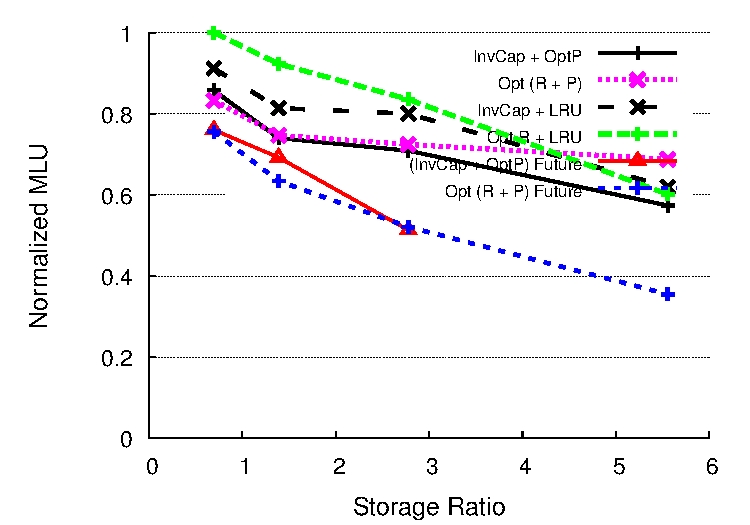
\includegraphics[scale=0.65]{graphSet1/singleoriginnew/ATTDownloads.pdf}}
\end{center}
\caption{Single origin node.}
\label{fig:singleorigin}
\end{figure*}


\begin{figure*}[t]
\begin{center}
\subfigure[News trace - Abilene] {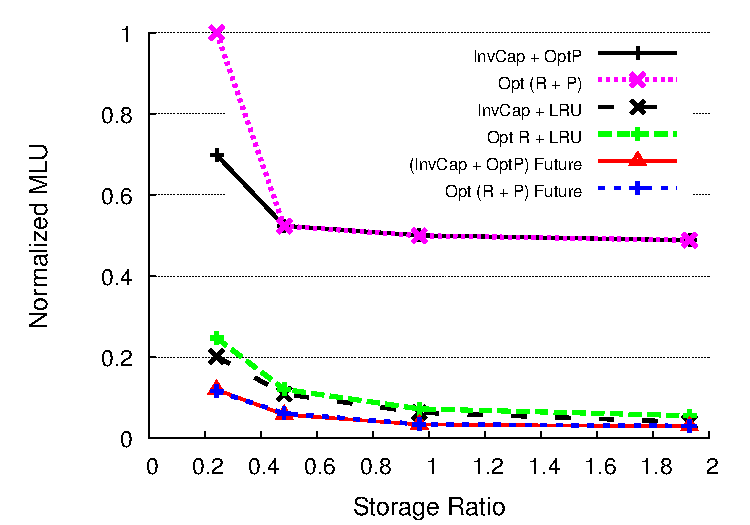
\includegraphics[scale=0.65]{graphSet1/fiveorigins/AbileneNews.pdf}}
\subfigure[News trace - ATT] {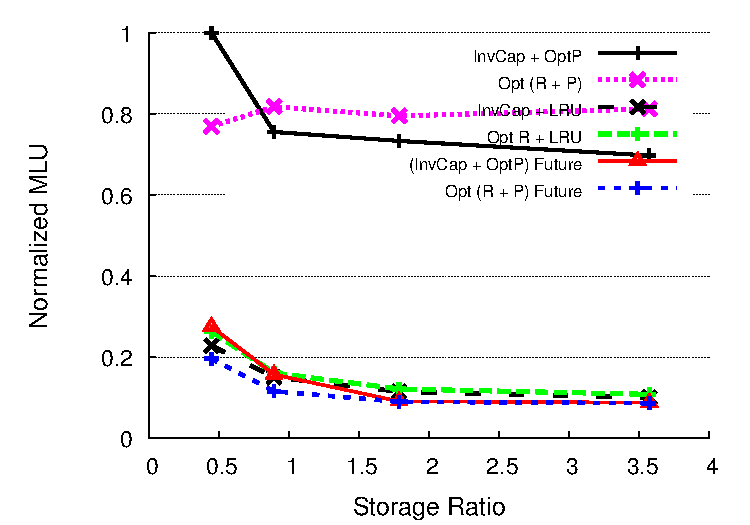
\includegraphics[scale=0.65]{graphSet1/fiveorigins/ATTNews.pdf}}
\subfigure[Entertainment trace - Abilene] {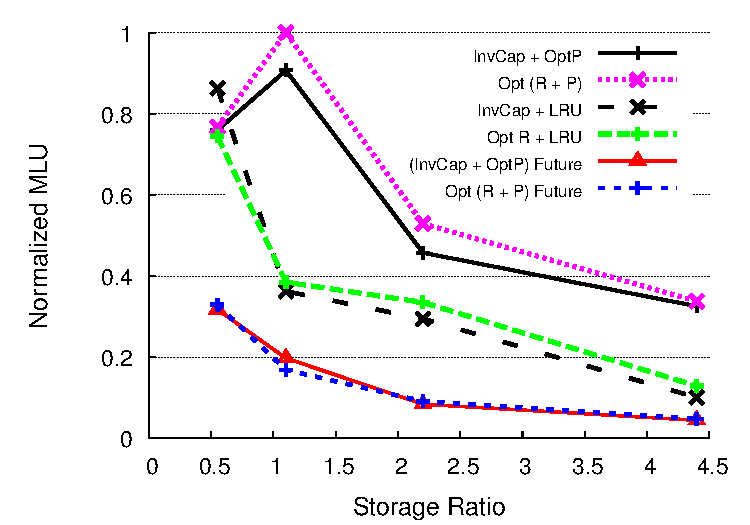
\includegraphics[scale=0.65]{graphSet1/fiveorigins/AbileneVideos.pdf}}
\subfigure[Entertainment trace - ATT] {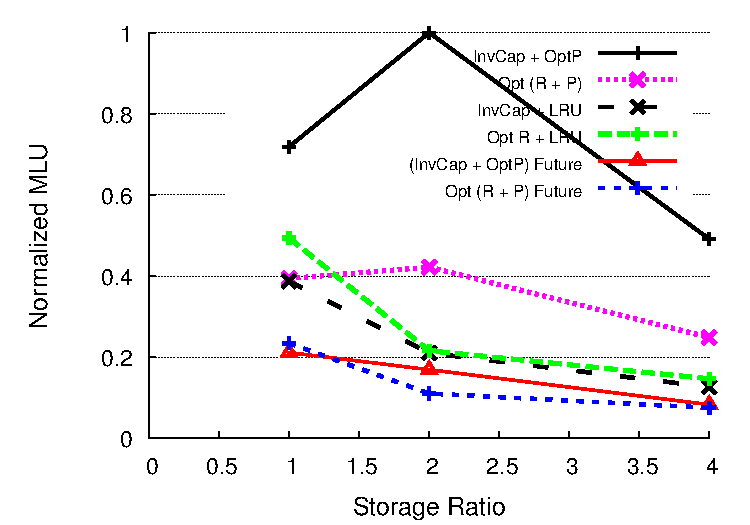
\includegraphics[scale=0.65]{graphSet1/fiveorigins/ATTVideos.pdf}}
\subfigure[Downloads trace - Abilene] {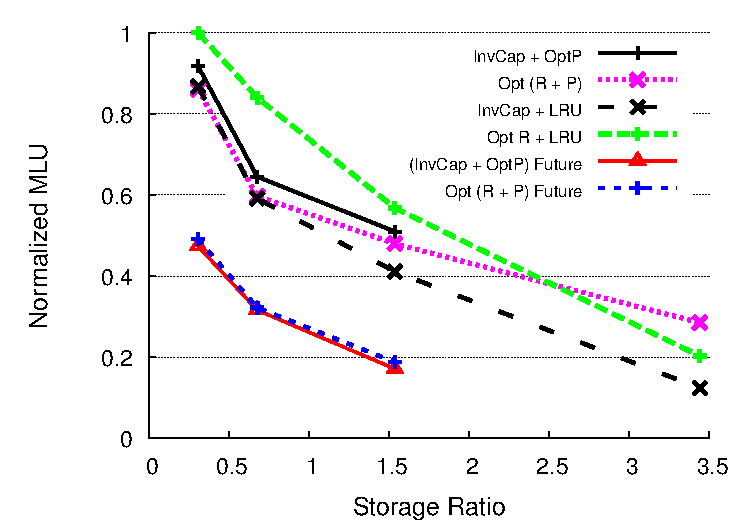
\includegraphics[scale=0.65]{graphSet1/fiveorigins/AbileneDownloads.pdf}}
\subfigure[Downloads trace - ATT] {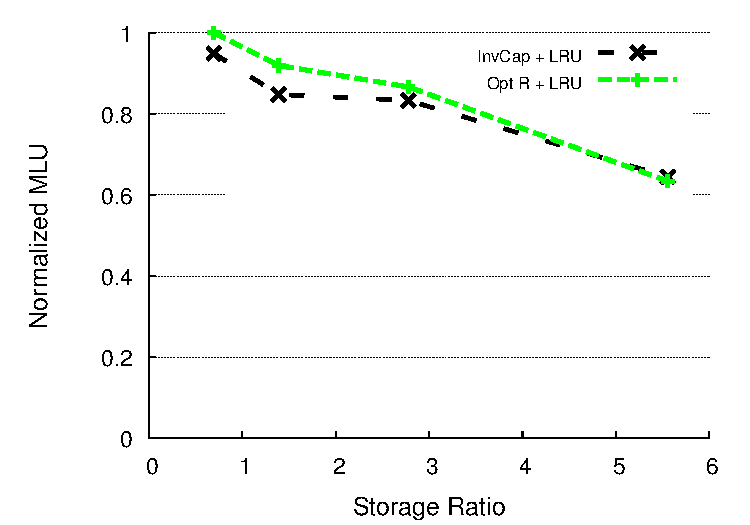
\includegraphics[scale=0.65]{graphSet1/fiveorigins/ATTDownloads.pdf}}
\end{center}
\caption{Five origin nodes.}
\label{fig:fiveorigins}
\end{figure*}

}

%Next, we varie two experiments: (1) We reduced the number of exit locations from three to one. (2) We increased the number of exit locations from three to five. 

%For both topologies, two locations are on the east coast and west coast respectively and the third location is in the central part of the US.  Now we explore the effect of increasing/decreasing the number of exit locations for traffic going to the origin server. For the first experiment, we assumed that all traffic going to the origin exits the network at only the central  location, excluding west coast and east coast locations. For the second experiment, we added two more exit locations - one from the eastern half of the map and other from the western half.

\subsubsection{Redirection Schemes for LRU}

\label{sec:redirectlru}
A demand-oblivous placement, LRU, specifies a cache replacement strategy, but there are several request redirection schemes that can be used in combination with LRU. In this section, we first propose a novel redirection scheme  that performs request redirection considering link utilizations in order to reduce network cost.  Next, we analyze whether requests should be redirected to all PoPs or a smaller subset of them in order to minimize network cost. We use content chunking for all experiments.
% as it improves performance of demand-oblivious placement.


\begin{figure}[t]
\begin{center}
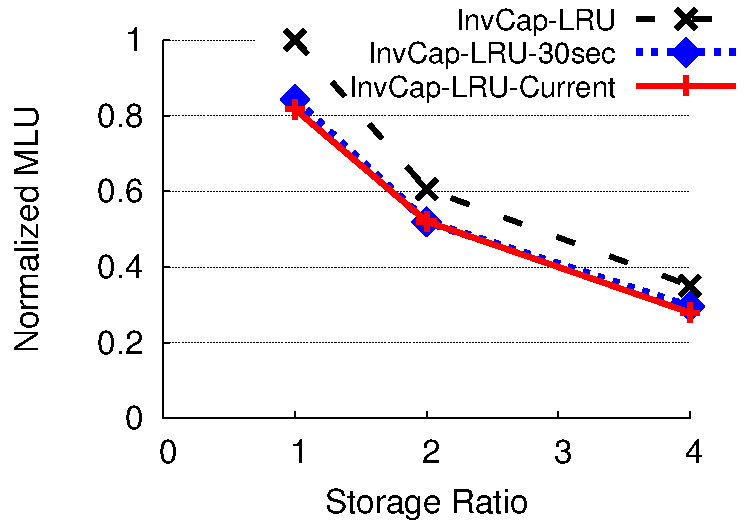
\includegraphics[scale=0.6]{graphSet1/lrusnmp/ATTVideos.pdf}
\end{center}
\caption{Link utilization aware request redirection helps \invlru\ reduce network cost up to 21\%. Link utilizations updated every 30 seconds performs as well as using current link utilizations. (Entertainment trace, AT\&T)}
\label{fig:lrusnmp}
\end{figure}




%A demand-oblivous placement, LRU, specifies a cache replacement strategy, but there are several request redirection strategies that can be used in combination with LRU. In this section, we explore two such strategies. The first strategy uses link utilization information to make a more informed request redirection decision. The second strategy redirects requests only to a small subset of PoPs unlike our current implementation which redirects requests to all PoPs. We use content chunking for all experiments as it improves performance of demand-oblivious placement.



\eat
{
\begin{figure*}[t]
\begin{center}
\subfigure[News trace - Abilene] {\includegraphics[scale=0.65]{graphSet1/lrusnmp/AbileneNews.pdf}}
\subfigure[News trace - ATT] {\includegraphics[scale=0.65]{graphSet1/lrusnmp/ATTNews.pdf}}
\subfigure[Entertainment trace - Abilene] {\includegraphics[scale=0.65]{graphSet1/lrusnmp/AbileneVideos.pdf}}
\subfigure[Entertainment trace - ATT] {\includegraphics[scale=0.65]{graphSet1/lrusnmp/ATTVideos.pdf}}
\subfigure[Downloads trace - Abilene] {\includegraphics[scale=0.65]{graphSet1/lrusnmp/AbileneDownloads.pdf}}
\subfigure[Downloads trace - ATT] {\includegraphics[scale=0.65]{graphSet1/lrusnmp/ATTDownloads.pdf}}
\end{center}
\caption{Link utilization aware request redirection helps \invlru\ reduce network cost up to 15\%-21\%. Link load information updated every 30 seconds performs as well as using current link load information.}
\label{fig:lrusnmp}
\end{figure*}
}

%\begin{figure}[t]	
%\begin{center}
%	\includegraphics[scale=1]{graphSet1/lrusnmp/mluincrease.png}
%\end{center}
%\caption{Link-load aware request redirection helps \invlru\ reduce network cost up to 27\%.}
%\label{fig:reqRedir}
%\end{figure}

%In order to reduce network cost, NCDN can use link load information which can be collected using SNMP protocol to make request redirection decisions. 
%A simple approach which we implement is following:  if a user's request results in a cache miss at the local PoP, we fetch content from other PoPs  which may have the content available. If multiple PoPs have the content, we choose that PoP for which the utilization of the most utilized link  along the path from that PoP to the local PoP is the least. We break ties based on hop count distance and then randomly.
%
%
%We have seen that a demand-oblivious placement and routing, i.e., \invlru\ performs well. In case of a cache miss, \invlru\ fetches content from other PoPs in the network which may have the content available. While a \invlru\ 
%
%\invlru\ serves a high 
%
%\invlru's performance can potentially be improved if 
%
%While \invlru\ scheme does not require 
%
%We have seen that \invlru\ scheme performs well 

\textbf{Link utilization aware request redirection:}
\label{fig:linkloadredir}
This scheme is designed to reduce link utilization in an NCDN. The idea is to periodically measure  utilizations of all links and then  redirect requests over the paths that have less utilized links. For example, if a request can be redirected to either of two PoPs, but the links along the path from one of the PoPs are more utilized than the links along the path from the other PoP, then the PoP whose path has \emph{less} utilized links is chosen. Compared to our current redirection strategy, i.e., choose the closest PoP based on hop count distance,  we expect that request redirection considering link utilizations will achieve lower network cost.

%Our intuition is that if \invlru\ does request redirection considering link utilization values, it can achieve a lower network cost compared to its default behavior, i.e., request redirection to the closest PoP based on hop count distance. 


%Link utilization values, which are necessary for this scheme, can be collected by an NCDN because it has access to network information. 


%In order to reduce link utilization, an NCDN can make request redirection decisions considering the current link utilization values. 


% The key idea is to redirect requests so that traffic flows along links that are least utilized as per the most recent measurements. Our intuition is that request redirection considering link utilization values can achieve a lower network cost compared to LRU's default behavior, i.e., request redirection to the closest PoP based on hop count distance. An NCDN can measure link utilization values  because it owns the network. 




% In this experiment, we evaluate a variant of \invlru\ which does request redirection using periodically measured link utilization values. Our intuition is that if \invlru\ does request redirection considering link utilization values, it can achieve a lower network cost compared to its default behavior, i.e., request redirection to the closest PoP based on hop count distance. Link utilization values, which are necessary for this scheme, can be collected by an NCDN by using SNMP protocol.

%In this experiment, we evaluate a variant of \invlru\ which does request redirection using periodically measured link utilization values. Link utilization values, which are necessary for this scheme, can be collected by an NCDN by using SNMP protocol. Our intuition is that if \invlru\ does request redirection considering link utilization values, it can achieve a lower network cost compared to its default behavior, i.e., request redirection to the closest PoP based on hop count distance.


Our implementation works as follows. When a request results in a cache miss at the local PoP (the PoP first contacted by a user), it fetches content from other PoPs  which may have the content available. If multiple PoPs have the content, the local PoP  fetches content from the PoP for which the utilization of the most utilized link  along the path from that PoP to the local PoP is the least. We break ties based on hop count distance and then randomly.


We experiment with two versions of the above algorithm, which differ in the frequency at which link utilizations are updated across all PoPs. In the first version, \textsf{\invlru-Current}, all PoPs in the network know the link utilizations  of all links at every moment. Clearly, this scheme represents the ideal case. In the second version, \textsf{\invlru-30sec}, link utilization is measured at all links every 30 seconds, and is updated across all PoPs. Our baseline for comparison is \invlru\ scheme. The exact frequency at which link utilizations are updated will depend on the implementation and is beyond our scope. 




Our results show that request redirection using link utilizations reduces network cost compared to \invlru.   
Figure \ref{fig:lrusnmp} presents the results for the experiment with entertainment trace on AT\&T topology (other graphs omitted for brevity).  \textsf{\invlru-Current} reduces network cost up to 19\% compared to \invlru.  On our experiments with other traces (graphs omitted), we find that \textsf{\invlru-Current} reduces network cost by 15\% to 21\% compared to \invlru.  In addition,  \textsf{\invlru-30sec} matches the network cost of \textsf{\invlru-Current} on all traces except for downloads trace on Abilene topology, where its network cost is higher by up to 9\%. This result implies that an implementation in which link utilization are updated at PoPs every 30 seconds can achieve most of the benefits of link utilization aware request redirection. 

%, and \textsf{\invlru-30sec}  achieves nearly the same network cost  as \textsf{\invlru-Current}

%achieves the same network cost on most traces as the ideal scheme in which PoPs know link utilization values at every moment.
 

%We present our results for this experiment  in Figure \ref{fig:lrusnmp}. 


%Therefore, request redirection using link utilization values reduces network cost for \invlru.  Moreover, an implementation in which link utilization values are updated at PoPs every 30 seconds achieves the same network cost on most traces as the ideal scheme in which PoPs know link utilization values at every moment.






%In this experiment, we show how a link load aware redirection strategy can further improve \invlru's performance. To this end, we evaluated its performance  with the following request redirection strategy which does not require link load information. If content is available at multiple PoPs in the network, we fetch the content from the PoP which is closest based on hop count distance, breaking ties randomly among PoPs with equal hop count distance. 
%
%We calculate the increase in MLU with the link load unaware request redirection strategy for each storage ratio we considered in our experiments in $\S$\ref{sec:video} and  $\S$\ref{sec:downloads}. In Figure \ref{fig:reqRedir}, we show the maximum and minimum reduction in MLU across all storage ratios for each CDN trace and network topology. Without a link load aware request redirection, \invlru\ has up to 38\% higher network cost. The maximum increase is nearly 35\% in all cases.
%
%Thus, using the recent link load information available to an NCDN can significantly reduce network cost for \ancp.


%For each storage ratio we considered in our experiments in $\S$\ref{sec:video} and  $\S$\ref{sec:downloads}, we calculated the increase in the MLU if with 



%\textbf{Less Cooperation among Caches:}
%\paragraph{Experiments with ``Neighbor-only'' LRU}


\begin{figure}[t]
\begin{center}
\includegraphics[scale=0.6]{graphSet1/lrulocalnew/AbileneDownloads.pdf}
\end{center}
\caption{\textsf{\invlru-Nbrs} redirects requests only to neighbors while \textsf{\invlru-Local} redirects to no other PoPs and sends requests directly to the origin. 
\textsf{\invlru-Nbrs} has a network cost within 27\% of \invlru\ while \textsf{\invlru-Local} incurs up to a 100\% higher network cost. (Downloads trace, Abilene) }
\label{fig:lrulocalnew}
\end{figure}

\textbf{Request redirection to neighbors:} 
%While our LRU implementation, redirects requests to all PoPs on a cache miss. 
In our \invlru\ implementation, a PoP redirects request to all PoPs on a cache miss, which maximizes the hit rate of network caches and reduces load on origin servers. To examine whether request redirection to all PoPs is necessary and to quantify its benefit on network cost, we compare  \invlru\ against two strategies that redirect requests to a much smaller set of PoPs. First is \textsf{\invlru-Nbrs}, in which a PoP redirects requests only to its one-hop neighbors on a cache miss before contacting the origin. Second is \textsf{\invlru-Local}, in which a PoP sends requests to the origin on a cache miss at a PoP. 



%In our \ncp\ architecture, a PoP requests content from all other PoPs on a cache miss before it contacts the origin. In this experiment, we ask if we restrict the number of PoPs contacted on a cache miss, what is its effect on the network cost.  Our objective is to evaluate the benefit of co-operation among PoPs and to examine if co-operation among all  PoPs in the network is necessary.


%We experimented with two variants of \invlru\ which unlike \invlru,  contact much smaller number of PoPs on a cache miss before they contact the origin. These are: (1) \textsf{\invlru-Nbrs}: A PoP redirects requests only to its one-hop neighbors on a cache miss before contacting the origin. (2) \textsf{\invlru-Local}: A PoP contacts the origin on a cache miss.


In Figure  \ref{fig:lrulocalnew}, we see that \textsf{\invlru-Nbrs} has a up to  to 6\% to 27\% higher network cost than \invlru\ depending on trace and topology. In comparison, \textsf{\invlru-Local} has up to 25\% to 100\% higher network cost than \invlru.  These results show that request redirection to other network caches helps reduce network cost, but most of this reduction can be had by redirection requests only to neighboring PoPs. 


%These results suggest that if a PoP does not communicate with any other PoP, s do not cooperate, then it can result in a significantly higher network cost. But, if PoPs co-operate only with their neighboring PoPs, they still can provide most of the reduction in network cost due to co-operation among all PoPs. 

\textsf{\invlru-Local}  serves up to 3$\times$ to $7\times$ more requests from origin than \invlru, which increases the utilization of links near the exit nodes connecting to origin nodes. 
\textsf{\invlru-Nbrs} also serves more requests from origin than \invlru, but the increase is up to 2$\times$ to 3$\times$ only. Therefore, network cost for \textsf{\invlru-Nbrs} is smaller compared to \textsf{\invlru-Local}.



\eat
{
We show the results in Figure \ref{fig:lrulocalnew}. \textsf{\invlru-Nbrs} has a up to  to 6\% to 25\% higher network cost than \invlru\ depending on trace and topology. In comparison, \textsf{\invlru-Local} has up to 25\% to 100\% higher network cost than \invlru.  These results suggest that if PoPs do not cooperate, then it can result in a significantly higher network cost. But, if PoPs co-operate only with their neighboring PoPs, they still can provide most of the reduction in network cost due to co-operation among all PoPs. 


\textsf{\invlru-Local}  sends up to 3$\times$ to $7\times$ serves more requests from origin than \invlru, which increases the utilization of links near the exit nodes in transit to the origin. 
\textsf{\invlru-Nbrs} also serves more requests from origin than \invlru, but the increase is up to 2$\times$ to 3$\times$. Therefore, network cost for \textsf{\invlru-Nbrs} is smaller compared to \textsf{\invlru-Local}.

}


%In this section, we experiment with a version of LRU which sends request only to its neighboring nodes instead of all the nodes in the network. Clearly, Local-LRU is easier to implement in practice since it requires responses from fewer number of nodes in the network. We experiment with two versions of this scheme -  InvCap+LRU Local and InvCap+LRU Local SNMP. While both these scheme send requests only to neighbors in case of a cache miss,  InvCap+LRU Local  uses the default request redirection strategy and InvCap+LRU Local SNMP  uses link load aware redirection strategy described in $\S$\ref{fig:linkloadredir}. 

%InvCap + LRU Local scheme incurs a  maximum increase  in MLU of 25\% over \invlru\ scheme, but the increase in MLU is less than 15\% at higher storage ratios. Since InvCap + LRU Local  is simpler to implement than \invlru, we believe \ancp\ should consider using InvCap + LRU Local instead of \invlru.

%In contrast, InvCap+LRU Local SNMP incurs up to 35\% higher MLU than InvCap+LRU SNMP. Thus, InvCap+LRU Local  scheme benefits much less from a  link load aware redirection strategy.



%\invlru's performance with varying levels of cooperation among caches. \invlru\ co-operates with caches at all PoPs, \invlru\ - Nbrs co-operates with caches at neighboring PoPs , \invlru\ - Local does not co-operate with any cache. \invlru\ - Nbrs has a network cost within 25\% of \invlru\ while \invlru\ - Local incurs up to a 100\% higher network cost.

\eat
{
\begin{figure*}[t]
\begin{center}
\subfigure[News trace - Abilene] {\includegraphics[scale=0.65]{graphSet1/lrulocalnew/AbileneNews.pdf}}
\subfigure[News trace - ATT] {\includegraphics[scale=0.65]{graphSet1/lrulocalnew/ATTNews.pdf}}
\subfigure[Entertainment trace - Abilene] {\includegraphics[scale=0.65]{graphSet1/lrulocalnew/AbileneVideos.pdf}}
\subfigure[Entertainment trace - ATT] {\includegraphics[scale=0.65]{graphSet1/lrulocalnew/ATTVideos.pdf}}
\subfigure[Downloads trace - Abilene] {\includegraphics[scale=0.65]{graphSet1/lrulocalnew/AbileneDownloads.pdf}}
\subfigure[Downloads trace - ATT] {\includegraphics[scale=0.65]{graphSet1/lrulocalnew/ATTDownloads.pdf}}
\end{center}
\caption{\invlru's performance with varying levels of cooperation among caches. \invlru\ co-operates with caches at all PoPs, \invlru\ - Nbrs co-operates with caches at neighboring PoPs , \invlru\ - Local does not co-operate with any cache. \invlru\ - Nbrs has a network cost within 25\% of \invlru\ while \invlru\ - Local incurs up to a 100\% higher network cost.}
\label{fig:lrulocalnew}
\end{figure*}
}

%\begin{figure*}[t]
%\begin{center}
%\subfigure[Entertainment trace - Abilene] {\includegraphics[scale=0.50]{graphSet1/lrulocal/AbileneVideos.pdf}}
%\subfigure[Entertainment trace - ATT] {\includegraphics[scale=0.50]{graphSet1/lrulocal/ATTVideos.pdf}}
%\subfigure[Downloads trace - Abilene] {\includegraphics[scale=0.50]{graphSet1/lrulocal/AbileneDownloads.pdf}}
%\subfigure[Downloads trace - ATT] {\includegraphics[scale=0.50]{graphSet1/lrulocal/ATTDownloads.pdf}}
%\end{center}
%\caption{Experiments with LRU Local.}
%\label{fig:lrulocal}
%\end{figure*}



%If content is present at multiple locations in the network, then LRU-SNMP chooses the location, for which the most utilized link  along the path from that location to the requesting PoP  has the smallest value. The current implementation has the accurate knowledge of utilization of all links at each time.  

\subsubsection{Is Traffic Engineering Necessary?}


\begin{figure}[t]
\begin{center}
\subfigure[News trace - Abilene] {\includegraphics[scale=0.5]{graphSet1/linkfailurecompare/AbileneNews.pdf}}
%\subfigure[News trace - ATT] {\includegraphics[scale=0.65]{graphSet1/linkfailure/ATTNews.pdf}}
\subfigure[Entertainment trace - Abilene] {\includegraphics[scale=0.5]{graphSet1/linkfailurecompare/AbileneVideos.pdf}}
%\subfigure[Entertainment trace - ATT] {\includegraphics[scale=0.65]{graphSet1/linkfailure/ATTVideos.pdf}}
%\subfigure[Downloads trace - Abilene] {\includegraphics[scale=0.65]{graphSet1/linkfailure/AbileneDownloads.pdf}}
%\subfigure[Downloads trace - ATT] {\includegraphics[scale=0.65]{graphSet1/linkfailure/ATTDownloads.pdf}}
\end{center}
\caption{Due to link failures, \invlru\ and \optrpfuture\ see up to  110\% and 99\% increase in MLU respectively. In case of link failures, \invlru\ can even achieve a lower network cost than \optrpfuture\ at high storage ratios.}
\label{fig:linkfailurecompare}
\end{figure}


Optimizing routing gives little improvement to network cost in an NCDN but this finding does not obviate traffic engineering by ISPs. The primary reason ISPs need traffic engineering is that they route transit traffic in addition to NCDN traffic. Since an ISP does not control either content placement or request redirection for transit traffic, traditional traffic engineering methods, e.g., OSPF traffic engineering, can reduce the network cost due to transit traffic.

Minimizing network cost in case of link failures is another objective of traffic engineering. Next, we study whether a demand-oblivious placement and routing, \invlru, that is highly effective in the failure-free scenario, also provides resilience to link failures. To this end, we compare performance of \invlru\ and \optrpfuture\  in case of link failures. The set of failure scenarios we consider includes all single link failures. We calculate the network cost for a failure scenario by simulating the entire trace with the failed link.  Among network costs for all failure scenarios, we select the highest network cost to compare the performance of a scheme.


%\noindent\emph{Topology Changes:} How do \invlru\ and \optrpfuture\ compare in case of topology changes caused by link failures ?


%Next, we experiment with link failures.   For each link failure, we calculate the network cost over the entire trace. Finally, we select the highest network cost among network costs for all failure scenarios. 



For this experiment, we added a constraint to \optrpfuture\ which ensures that the set of paths between any pair of nodes has at least two paths with no links in common. As a result, the routing computed is resilient to any single link failure. In terms of variables in Table \ref{table:paramtable}, our constraint is 

\begin{center}
$f_{ije} \leq \beta \times f_{ij}, \quad \forall e \in E, i,j \in V $
\end{center}

\noindent where we set $\beta = 0.75$. This constraint means that a link can carry at most 75\% of traffic between any pair of nodes. \optrpfuture\ calculates placement and routing assuming a failure-free scenario. In case of a link failure, we update routing by excluding all paths that cross the failed link. For each pair of nodes, traffic splitting ratios for the working paths are multiplied by a normalizing constant such that traffic splitting ratios add up to one. \invlru\ updates shortest path routes in case of a link failure while keeping link weights the same.




In Figure  \ref{fig:linkfailurecompare}, we show the network cost of \invlru\ and \optrpfuture\ in failure-free scenario and their network costs during failures. Both \invlru\ and \optrpfuture\ see up to 110\% and 99\% increase in network cost  respectively during failures.  During failures we find that \invlru\  has a significantly higher network cost than \optrpfuture\  at small storage ratios, but the difference reduces at higher storage ratios with \invlru\ even achieving a lower network cost than \optrpfuture\ at the maximum storage ratio in each graph.  Comparing the failure-free scenario and link failure scenarios, the relative sub-optimality of \invlru\ with respect to \optrpfuture\ remains the same at small storage ratios or but reduces at higher storage ratios. The nonmonotonicity of \optrpfuture\ is because it optimizes routing and placement assuming a failure-free scenario and hence performs sub-optimally when link failures occur. We believe that our analysis of the network cost during failures could be further improved, e.g., we  consider only the worst case network cost in case of link failures, and our modification of \optrpfuture\ does not provide a  guarantee that the modified routing will be optimal in case of link failures.

%Therefore, compared to failure-free scenario, the relative sub-optimality of \invlru\ with respect to \optrpfuture\ remains the same at small storage ratios or but reduces in case of link failures. 



%that is equal to inverse of the sum of traffic splitting ratios of working paths.

%We calculate network cost for \invlru\  on a link failure by simulating the trace on the ISP topology after removing the failed link. 

%In case of a link failure \invlru\ updates its the shortest path excluding the failed link. 

%\invlru\ works as follows in case of link failures. 

%We made one change to \optrpfuture\ so that it can withstand all single link failures. 

%For this experiment, we compared the performance of \invlru\ across all link failures.  Due to time constraints, simulating \optrpfuture\ for all link failures is not feasible, therefore we only present a comparison of \invlru\ with  \optrpfuture\ for the link failure scenario which results in the maximum MLU for  \invlru. 







%\begin{figure*}[t]
%\begin{center}
%\subfigure[News trace - Abilene] {\includegraphics[scale=0.65]{graphSet1/linkfailure/AbileneNews.pdf}}
%\subfigure[News trace - ATT] {\includegraphics[scale=0.65]{graphSet1/linkfailure/ATTNews.pdf}}
%\subfigure[Entertainment trace - Abilene] {\includegraphics[scale=0.65]{graphSet1/linkfailure/AbileneVideos.pdf}}
%\subfigure[Entertainment trace - ATT] {\includegraphics[scale=0.65]{graphSet1/linkfailure/ATTVideos.pdf}}
%\subfigure[Downloads trace - Abilene] {\includegraphics[scale=0.65]{graphSet1/linkfailure/AbileneDownloads.pdf}}
%%\subfigure[Downloads trace - ATT] {\includegraphics[scale=0.65]{graphSet1/linkfailure/ATTDownloads.pdf}}
%\end{center}
%\caption{Is \invlru\ resilient to link failures ? In the worst case, \invlru\ incurs a 66\% increase in MLU due to link failure on Abilene topology and a 200\% increase in network cost due to link failure on ATT topology.}
%\label{fig:linkfailure}
%\end{figure*}
